\section{THERMAL TRANSPORT IS INFLUENCE By NANOPARTICLE SHAPE}
%\begin{abstract}
\subsection{Abstract}
  Molecular dynamics simulations were performed to model the
  interfacial thermal conductance ($G$) from bare gold nanoparticles
  (icosahedral, cuboctahedral, and spherical) to a hexane
  solvent. The computed conductance was found to depend not only on
  particle shape, but also on the size of the nanoparticles,
  particularly for nanospheres.  These results are compared with
  conductance out of the planar facets: (111), (100), and (110);
  all commonly exhibited in small patches by the spherical
  particles. Undercoordination of the surface atoms and the
  vibrational density of states in the icosahedra explain some of
  these observations. The exposed surfaces of icosahedral particles
  are dominated by (111) facets with 9-coordinated gold atoms.
  Cuboctahedral particles are dominated by the (100) and (111) facets
  with 8- and 9-coordinated surface atoms, respectively.  The
  nanospheres approach a constant surface density of 6-9 coordinated
  sites at large particle sizes, and these surface atoms play a large
  role in the conductance to the solvent.  The surface-normal
  vibrational densities of states were used to explain a simple
  surface undercoordination model, which shows a size-dependent
  enhancement of low-frequency coupling to the solvent.
%\end{abstract}


%%%%%%%%%%%%%%%%%%%%%%%%%%%%%%%%%%%%%%%%%%%%%%%%%%%%%%%%%%%%%%%%%%%%%%%%%%%%%%%%%%%
%		INTRODUCTION
%%%%%%%%%%%%%%%%%%%%%%%%%%%%%%%%%%%%%%%%%%%%%%%%%%%%%%%%%%%%%%%%%%%%%%%%%%%%%%%%%%%
\subsection{Introduction}
Thermal transport between nanoparticles and their surrounding
environments depends on many factors, including particle
size,\cite{Zanjani2014,Liu2015,Wilhelmsen2015,Stocker2016,Tascini2016}
composition,\cite{Wilson:2002uq, Ge:2004,Ong:2013rt} surface
modification,\cite{Ge:2004,kuang:AuThl,Ong:2013rt,Ong:2014yq,Liu2015,Stocker2016,Hannah2015,Park2016,Meng:2017,Leitner2017}
surface supports,\cite{Schmidt:2010,Park2012} exposed surface
facets,\cite{Norris:2013,Hannah2015,Han:2017} and the chemical details
of the
environment.\cite{Ge2006,Schmidt:2010,Park2012,Ong:2013rt,Ong:2014yq,Wilhelmsen2015,Giri:2016,Park2016,Bhanushali:2017,Yadav:2017}
Particle morphology may also play a role in heat transfer out of
nanostructures.  This is the central question of this work -- all
other things being equal, will different particle morphologies yield
different heat transfer properties to the solvent?

Tascini \textit{et al.}\cite{Tascini2016} studied the
curvature dependence of the interfacial thermal conductance for
partially solvated nanospheres. They found an empirical relationship,
\begin{equation}
G(r) = G(\infty) + \frac{\delta}{r}
\label{Tascini}
\end{equation}
where $G(r)$ is the conductance out of a sphere of radius $r$,
$G(\infty)$ is a parameter describing the infinite-radius limit of the
conductance, and $\delta$ describes the approach to the infinite size
limit. Notably, the Tascini \textit{et al.} simulations predict a
positive $\delta$, where smaller particles exhibit high interfacial
thermal conductance and approach an infinite surface limit that has
lower thermal conductance to the solvent. This makes intuitive sense
-- one might expect the large particle limit to approach the behavior
of flat interfaces.

To test this hypothesis, heat transfer out of gold
nanospheres that were in direct contact with a molecular solvent have been computed. The
spheres were cut out of an infinite FCC lattice and spanned a range of
sizes.  The spheres
expose many surface facets including patches of the (111), (100), and
(110) facets, due to the cuts in the underlying FCC lattice.
The interfacial thermal conductance out of similarly-sized
 icosahedral particles that exhibit only (111) facets and cuboctahedral particles that display
only (111) and (100) facets have been compared to the spheres. 
I have also compared the interfacial thermal conductance to flat interfaces 
that match the facets exposed on the surfaces of the spheres.

One possible explanation for an empirical relationship like
Eq. (\ref{Tascini}) is that there is a significant contribution to
interfacial thermal conductance that depends on the surface area to
volume ratio, suggesting a large role for the surface atoms. In 
previous work, the thermal conductance out of chemically-modified gold
surfaces was examined via reverse nonequilibrium molecular dynamics
(RNEMD). \cite{kuang:AuThl,Stocker:2014qq,Stocker2016} %add citation
In these studies, surfactants attached to the gold surfaces contained
a strong gold -- sulfur interaction that acted as a bridge for
vibrational energy to travel to the ligand.  Although the presence and
density of the ligand layer has a large effect on the interfacial
conductance, no clear trend was established regarding the size and
curvature of the underlying nanoparticles. Previous studies from
Tascini \textit{et al.}\cite{Tascini2016} and Ong \textit{et
  al.}\cite{Ong:2014yq} predict a decrease in the interfacial thermal
conductance as the particle radius increases, although Ong \textit{et
  al.}\cite{Ong:2014yq} and Zanjani \textit{et al.}\cite{Zanjani2014}
predict higher thermal conductivity with increasing core diameter in
nanocrystal arrays. However, if surface modifications dominate
conductance, the presence of a moderate density of ligands will
obscure the effects of particle curvature.

\subsubsection{Size- and temperature-dependent particle morphologies}
The nanoparticles simulated for this work ranged in size from 309
atoms to 14,993 atoms.  Ercolessi \textit{et al.}\cite{Ercolessi1991}
annealed at temperatures from 400K to 1400K and found the dominant
structures for different sizes of gold particles
($N = 100 \text{-} 900$ atoms).  For $N = 100 \text{-} 200$, the
structures were dominated by glassy clusters while for
$N = 200 \text{-} 900$, the structures were predominantly
cuboctahedral. Similarly, Myshlyavtsev and Stishenko found, when
comparing gold nanostructures, a transition from a fully (111)
icosahedral structure to a (100)-terminated cuboctahedral structures
between 561 to 1,415 atoms, depending on the potential energy
function.\cite{Myshlyavtsev2013} Distinct vibrational densities of
states have also been observed for the cuboctahedral clusters relative
to icosahedra.\cite{Sauceda2015}

In a study of the thermal stability of gold icosahedra, Wang
\textit{et al.}\cite{Wang2004} found that softening of the vertex and
edge atoms occurs at $\approx$ 800K.  During this process they saw
enhanced surface atom diffusion due to the mobility of the vertex and
edge atoms.

The size range ($N = 300 \text{-} 15,000$) and temperatures (250K) for
the calculations described here exhibit stable icosahedra with
relatively low surface atom mobility, except for the smallest
($r = 18 \text{-} 22$~\AA) particles, which may be metastable relative to
cuboctahedra.

\subsubsection{Theory}
Under the diffuse mismatch model (DMM), the thermal conductance at an interface between $a$ and $b$ can be approximated,  
\begin{equation}
G_{ab} = \frac{1}{4 \pi} \sum_p \int_\omega \int_\theta \int_\phi \hbar \omega \frac{\partial f}{\partial T}  v_a  \rho_a  \tau_{ab} \cos\theta \sin\theta d\theta d\phi d\omega
\end{equation}
where $f$ is the Bose-Einstein distribution function, $v_a(\omega, p)$
is the group velocity (on side $a$) for a phonon characterized by
frequency $\omega$, moving in direction ($\theta, \phi$) with
polarization $p$.  The relevant material properties are the density of
phonon states, $\rho_a(\omega, p)$ and the transmission probability,
$\tau_{ab}(\omega, p)$, at the
interface.\cite{Swartz:1989uq,Reddy:2005fk,Monachon2016}
%The DMM also assumes that phonons scatter into states with the same frequency on either side, and that the scattering phonons lose memory of their incident angles.  This requires a symmetry in the transmission probabilities,
% \begin{equation}
% \tau_{ab}(\omega) = 1 - \tau_{ba}(\omega)
% \end{equation}

The diffuse mismatch model has a number of significant issues,
particularly when the Debye model is a poor representation of the
density of states, or where there is a fictitious boundary between
identical materials (where the DMM predicts a non-zero
resistance).\cite{Monachon2016} There is also an assumption of
detailed balance built-in to the model,\cite{Chen2005} which requires
the two sides to be at equilibrium.  This assumption is violated under
non-equilibrium conditions, as in the RNEMD simulations used
here. Although the DMM is not quantitative, it does suggest a role for
frequency-dependent phonon transmission at the interface and 
that isolating the frequencies of the phonons moving
towards the interface could aid in understanding interfacial
conductance. 

Using atomic velocities projected in a direction normal to the
interface,
\begin{equation}
v^{\perp}_i(t) = \mathbf{v}_i(t) \cdot \hat{\mathbf{n}}, 
\end{equation}
it is straightforward to compute vibrational power spectra,
\begin{equation}
  \rho^\perp (\omega) = \frac{1}{\tau} \int_{-\tau/2}^{\tau/2} \langle v^{\perp}(t) \cdot v^{\perp}(0) \rangle e^{-i\omega t} dt
\label{eq:DOS}
\end{equation}
which have been averaged over direction and polarization, where $\tau$
is the total observation time for the autocorrelation function.  
This can be used to approximate the density of phonon states of the two
materials near the interface, which can provide a clearer picture of
vibrational communication between the two materials. 
%We can also use information about the \textit{locations} of the vibrating atoms to arrive at a transmission model that gives a clearer picture of vibrational communication across the interface.
By further restricting the density of states calculation to specific
atoms at the metallic side of the interface, I hope to provide a
mechanism for heat flow from the solid and into the surrounding
liquid.

To compute interfacial thermal conductance values directly,
reverse non-equilibrium molecular dynamics (RNEMD)
simulations are utilized.\cite{Muller-Plathe:1997wq,Kuang:2012fe} RNEMD imposes an
unphysical kinetic energy exchange between the center of the particle
and a spherical shell of solvent that is well-separated from the
interface.  The system responds by creating a thermal gradient in the
metal and solvent regions, and a temperature discontinuity at the
interface between the particle and the solvent. The Kapitza resistance
of the interface,
\begin{equation}
  R_\mathrm{K} = \frac{1}{G} = \frac{1}{q_r} \sum_i \left(T_{i+i} - T_i\right) 4 \pi r_i^2,
  \label{sphericalG}
\end{equation}
is estimated by summing the individual thermal resistances of
concentric spherical shells as the radius
increases.\cite{Stocker:2014qq} Here, $T_i$ is the temperature of a
shell with radius $r_i$, and $q_r$ is the heat rate (the relevant
measure of thermal transport in spherical geometries). The heat rate
is the surface area of the particle times that of the imposed
flux. The interfacial thermal conductance of the interface, $G$ is the
inverse of the net Kapitza resistance.  For interfaces of appreciable
width, the relevant shells for measuring interfacial resistance are
the largest shell that is unambiguously in the particle and the
smallest shell that is unambiguously in the solvent.

For planar or periodic geometries, the interfacial thermal conductance
can be similarly computed by imposing a non-physical flux between two
separated slabs in the simulation cell. In this case, the Kapitza
resistance,
\begin{equation}
  R_\mathrm{K} = \frac{1}{G} = \frac{\Delta T}{J_z},
\label{planarG}
\end{equation}
depends on the imposed kinetic energy flux, $J_z$, in a direction
normal to the interface ($z$), and the steady-state temperature drop,
$\Delta T$, across the interface.\cite{Kuang:2012fe}

%%%%%%%%%%%%%%%%%%%%%%%%%%%%%%%%%%%%%%%%%%%%%%%%%%%%%%%%%%%%%%%%

\subsection{Computational Details}

Solvated gold nanoparticles ranging in diameter from 20-80 \AA\ were
simulated using reverse non-equilibrium molecular dynamics (RNEMD) in
a spherical shell of hexane. Similar planar systems, displaying (111),
(110), and (100) facets with hexane solvent were also prepared.  The
following sections describe the system composition, 
the potentials used to calculate the
interactions in the system, as well as the simulation protocol.

\subsubsection{System Composition}
Both the nanoparticle and planar systems contain only gold atoms and
hexane molecules.  The composition of the planar systems can be found
in Table \ref{tab:facet} and the nanoparticle system details can be
found in Tables \ref{tab:spheres}, \ref{tab:icosahedra}, and \ref{tab:cubos}.

\begin{table}
\centering
\caption{Composition of the solvated planar facet systems and the
  physical extent of the gold slabs ($L_x$, $L_y$, and $L_z$). The
  hexane molecules occupy the remainder of a 100 \AA\ box (length
  measured along the $z$-axis).
  \label{tab:facet}}
\begin{tabular}{ c|cccc| c }
\toprule
Facet & Au atoms & $L_x$ (\AA) &$L_y$ (\AA) & $L_z$ (\AA) & Hexane Molecules\\
\midrule
(111) &  972 & 25.915   & 29.888 & 18.952 & 284      \\
(110) & 1800 & 40.131   & 34.089 & 20.280 & 498      \\
(100) & 1008 & 24.322   & 24.382 & 26.422 & 200      \\
\bottomrule
\end{tabular}
\end{table}

\begin{table}
\centering
\caption{Composition of the solvated nanosphere simulations.
  \label{tab:spheres}}
\begin{tabular}{ c|cc }
\toprule
        & \multicolumn{2}{c}{Components}\\
Particle Radius (\AA) & Au atoms & Hexane Molecules \\
\midrule
 9.20 $\pm$ 0.28  & 249   &  2894      \\
14.30 $\pm$ 0.31  & 887   &  6304      \\
19.07 $\pm$ 0.28  & 1985  &  8555      \\
24.09 $\pm$ 0.32  & 3925  & 11576      \\
29.03 $\pm$ 0.29  & 6699  & 15376      \\
34.01 $\pm$ 0.32  & 10641 &  9235      \\
38.88 $\pm$ 0.31  & 15707 &  8056      \\
\bottomrule
\end{tabular}
\end{table}

\begin{table}
\centering
\caption{Composition of the solvated icosahedral nanoparticle simulations.
  \label{tab:icosahedra}}
\begin{tabular}{ cc|cc }
\toprule
       &            & \multicolumn{2}{c}{Components}\\
$n$ shells & radius (\AA) & Au atoms & Hexane Molecules \\
\midrule
4  &  9.45 $\pm$ 0.15  &   309 &  2894      \\
5  & 11.75 $\pm$ 0.17  &   561 &  4320      \\
6  & 14.07 $\pm$ 0.19  &   923 &  6304      \\
7  & 16.39 $\pm$ 0.21  &  1415 &  7414      \\
8  & 18.71 $\pm$ 0.25  &  2057 &  8555      \\
9  & 21.04 $\pm$ 0.27  &  2869 &  8555      \\
10 & 23.36 $\pm$ 0.30  &  3871 & 11576      \\
11 & 25.69 $\pm$ 0.32  &  5083 & 11576      \\
12 & 28.02 $\pm$ 0.35  &  6525 & 11576      \\
13 & 30.35 $\pm$ 0.38  &  8217 &  7741      \\
14 & 32.67 $\pm$ 0.41  & 10178 &  9235      \\
15 & 35.00 $\pm$ 0.43  & 12430 & 10911      \\
16 & 37.33 $\pm$ 0.66  & 14993 & 11576      \\
\bottomrule
\end{tabular}
\end{table}

\begin{table}
\centering
\caption{Composition of the solvated cuboctahedral nanoparticle simulations.
  \label{tab:cubos}}
\begin{tabular}{ c|cc }
\toprule
        & \multicolumn{2}{c}{Components}\\
 radius(\AA)      & Au atoms & Hexane Molecules \\
\midrule
 7.41 $\pm$ 0.35  &   147 & 11360      \\
10.16 $\pm$ 0.53  &   309 &  3387      \\
12.15 $\pm$ 0.50  &   561 &  5888      \\
14.98 $\pm$ 0.69  &   923 &  7414      \\
16.93 $\pm$ 0.65  &  1415 &  9440      \\
19.80 $\pm$ 0.85  &  2057 &  9380      \\
21.73 $\pm$ 0.82  &  2869 & 10317      \\
24.13 $\pm$ 0.90  &  3871 & 14185      \\
26.53 $\pm$ 0.99  &  5083 & 19585      \\
31.34 $\pm$ 1.15  &  8217 & 12626      \\
36.15 $\pm$ 1.32  & 12431 & 17457     \\
\bottomrule
\end{tabular}
\end{table}

Planar systems were constructed with the exposed $(hkl)$ facets
directed normal to the positive and negative $z$-axis.  The simulation
cell dimensions were set by the facet, and the simulation box was
enlarged along the $z$ dimension to a fixed size of 100 \AA.  The
remaining space was filled with hexane molecules to a density of
0.6548 $\text{g cm}^{-3}$.


%%%%%%%%%%%%%%%%%%%%%%%%%%%%%%%%%%%%%%%%%%%%%%%%%%%%%%%%%%%%%%%%%%%%%%%%%%%%%%%%%%%
%		FORCE FIELDS
%%%%%%%%%%%%%%%%%%%%%%%%%%%%%%%%%%%%%%%%%%%%%%%%%%%%%%%%%%%%%%%%%%%%%%%%%%%%%%%%%%%
\subsubsection{Force Fields}

For this work, gold -- gold interactions are calculated using the
quantum Sutton-Chen (QSC) model.\cite{Qi:1999ph} The hexane solvent is
described by the TraPPE united atom (UA)
model.\cite{TraPPE-UA.alkanes} The bonds in TraPPE-UA are rigid, but
here the bonds are made flexible using harmonic force constants
borrowed from OPLS-AA for intra-molecular sites closer than 3
bonds.\cite{Jorgensen98a} The interactions between Au atoms and atoms
on the hexane molecules were fit to a pairwise Lennard-Jones
potentials based on a study by Hautman and Klein for Au(111)
surfaces.\cite{hautman:4994} Details of the interaction potentials are
identical to previous work and previous chapter on heat 
transport for thiolate-protected gold nanospheres.\cite{Stocker2016}

%%%%%%%%%%%%%%%%%%%%%%%%%%%%%%%%%%%%%%%%%%%%%%%%%%%%%%%%%%%%%%%%%%%%%%%%%%%%%%%%%%%
%		SIMULATION PROTOCOL
%%%%%%%%%%%%%%%%%%%%%%%%%%%%%%%%%%%%%%%%%%%%%%%%%%%%%%%%%%%%%%%%%%%%%%%%%%%%%%%%%%%
\subsubsection{Simulation Protocol}
The gold nanospheres were prepared by cutting a FCC lattice with radii ranging
10 - 40 \AA. 
Icosahedral particles were
constructed in nested shell structures, built around an ideal
icosahedral core.  Cuboctahedral particles were built by cutting (111)
and (100) facets from a FCC lattice.
All particles were thermally equilibrated before being
solvated with thermally equilibrated hexane using packmol.\cite{packmol}
Once solvated, the systems were equilibrated for a minimum of 1 ns 
using the Langevin Hull 
integrator with an external bath characterized by 50 atm of
pressure and a temperature bath at 250K.\cite{Vardeman2011}
Random seeds were used in both the packing of the solvent and the equilibration process to ensure independent samples.

Planar interfaces displaying the Au(111), Au(110), and Au(100) facets
were prepared as slabs $\sim$ 20 \AA\ thick with the relevant facets
rotated normal to the $z$-axis. Surface stress was removed by relaxing
the systems for 1 ns at 250 K in a constant surface tension
(N\(\gamma\)T) ensemble with zero applied surface tension, followed by
1 ns in the microcanonical (NVE) ensemble.  Hexane molecules were
packed into the remaining box volume with a density of 0.6548
g/cm$^3$. The solvated systems were then equilibrated using the
canonical (NVT) ensemble at 250 K for 1 ns followed by further
relaxation in the microcanonical ensemble for 1 ns.

Following equilibration, the relevant thermal flux was applied for 1
ns for the nanoparticle systems and 3 ns for the planar systems,
allowing for a steady-state temperature gradients to develop. Mean
temperatures of the system remained at 250K, preserving the solvent
cluster around the nanoparticles and preventing the formation of a
vapor layer. Thermal coupling to the external temperature bath was
removed to avoid interference with the imposed flux. The metal
particles equilibrated rapidly, and were typically found with elevated
temperatures ($\sim$300K) relative to the bulk. Because the solvent
volume is large relative to the particles, the solvent finds a steady
state temperature just below 250K throughout most of the
volume. Adjacent to the surface of the particles, solvent temperatures
are typically close to 260K. The TraPPE-UA hexane model boils at
$\sim$ 330K, so the simulation conditions are reasonable for
maintaining liquid surroundings for the particles.  All simulations
were carried out with the open source molecular dynamics package,
OpenMD.\cite{openmd,OOPSE}

Five separate configurations for each system size were simulated to
provide statistical independence of the hexane packing.  Thermal
conductance was calculated using the same methods found in Stocker
\textit{et al.}\cite{Stocker2016} for the non-periodic systems and for
the planar systems.\cite{Stocker:2013cl}

\subsection{Results and Discussion}
The interfacial thermal conductance ($G$) for hexane-solvated
spherical, icosahedral, and cuboctahedral Au nanoparticles was
computed using RNEMD simulations, and was compared with the same
quantity for a series of planar gold interfaces, including the
Au(111), Au(100), and Au(110) interfaces.  These surfaces are all
exhibited as microfacets on the surfaces of the nanospheres, and the
Au(111) facet is the primary facet displayed by the icosahedra,
where the cuboctahedra display Au(111) and Au(100).

Computed interfacial thermal conductance values for the icosahedra,
cuboctahedra, nanospheres, and flat facets are shown in
Fig. \ref{fig:ico_vs_sphere}.  The nanospheres have a pronounced
dependence on the particle radius, $r$, while the icosahedral
conductance stays relatively close to the value obtained for the
Au(110) facet. Thermal transport out of the cuboctahedral particles
show a mostly linear dependence on particle radius.  The smooth line
going through the conductance values for the spheres is a fit using
the Tascini \textit{et al.}\cite{Tascini2016} model
(Eq. (\ref{Tascini})) with
$G(\infty) = 49.25~\text{MW}~\text{m}^{-2}~\text{K}^{-1}$, and
$\delta = -156.25~\text{MW \AA}~\text{m}^{-2}~\text{K}^{-1}$.
Notably, our simulations project a value for the interfacial
conductance of the infinite spheres that is significantly
\textit{higher} than many of the flat facets.  To explain this
observation, the surface density of undercoordinated atoms
and the vibrational densities of states of these undercoordinated
atoms are discussed in the following sections.

\begin{figure}
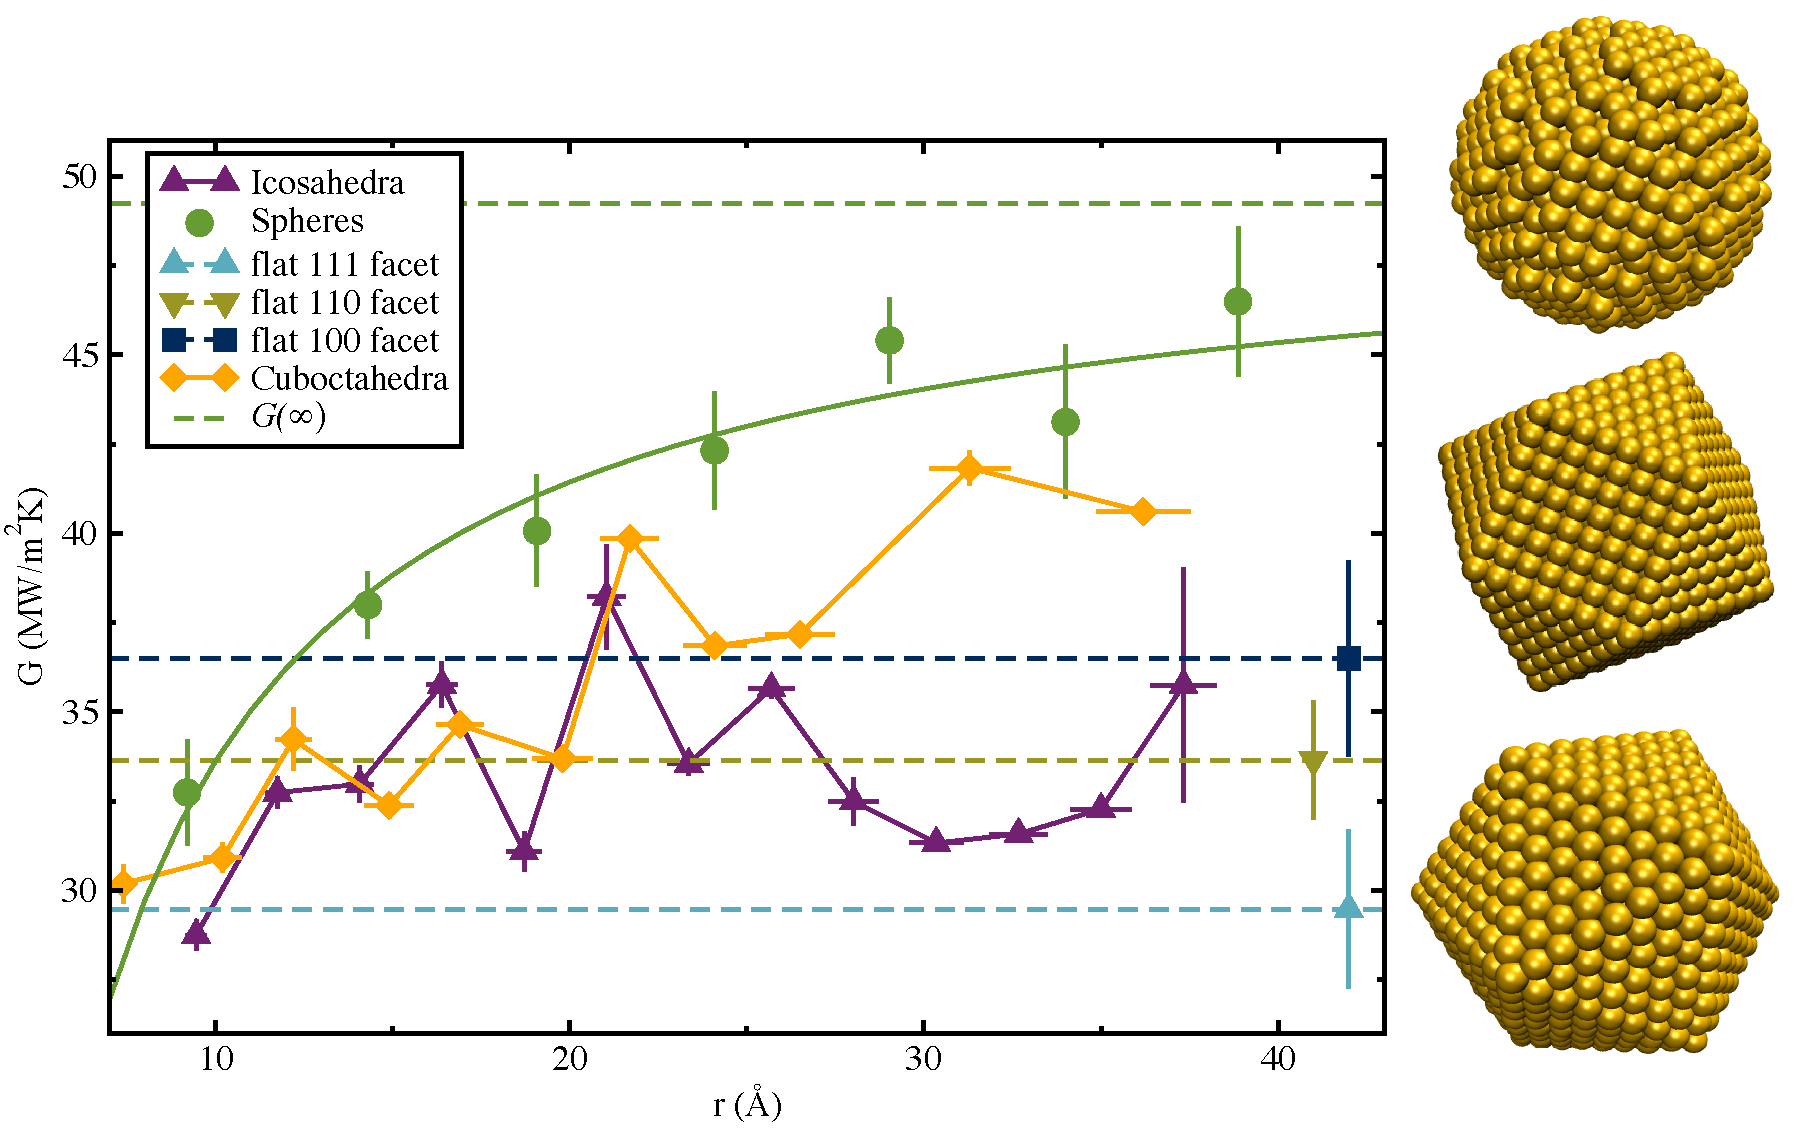
\includegraphics[width=\linewidth]{figures/g-ico-spher-cub.pdf}
	\caption{Interfacial thermal conductance, $G$, for bare gold
          nanospheres, cuboctahedra, and icosahedra in contact with
          hexane solvent. Conductances for flat Au(111), Au(100), and
          Au(110) interfaces are indicated with dashed horizontal
          lines.  A fit using the model of Tascini \textit{et al.} is
          shown along with the predicted value of $G(\infty)$, the
          infinite particle limit.}
	\label{fig:ico_vs_sphere}
\end{figure}

The spherical particles display all three of the planar facets (as
well as small regions of higher index facets), and for most of the
size range simulated, they also exhibit a significantly higher
interfacial thermal conductance than the low-index facets.

For icosahedral particles, there is no clear dependence of $G$ on the
particle size, and the larger particles exhibit thermal conductance
values slightly above the expected (111) conductance for particles
with $r \approx 35$ \AA. There is some instability in the values of
$G$ in the range of $r = 18-22$ \AA, which is near the 
transition from stable icosahedra to
cuboctahedra.\cite{Myshlyavtsev2013}

\subsubsection{Hexane Density}
The hexane density as function of distance from the gold at the
interface of the planar facets is provided in Fig. \ref{fig:dens}. The
solvent in the (111) and (100) systems display similar behavior, while
the solvent near the (110) interface comes closer to the surface
atoms.  In the (110) system, the first layer of hexane is spread out
over a thicker slab in comparison to the other two systems and allows
solvent to come closer to the interfacial atoms.  This is likely due
to the ridges present on this interface.  Within 5 \AA\ of the
interfacial gold layer, the three systems have the same amount of
hexane.

\begin{figure}
        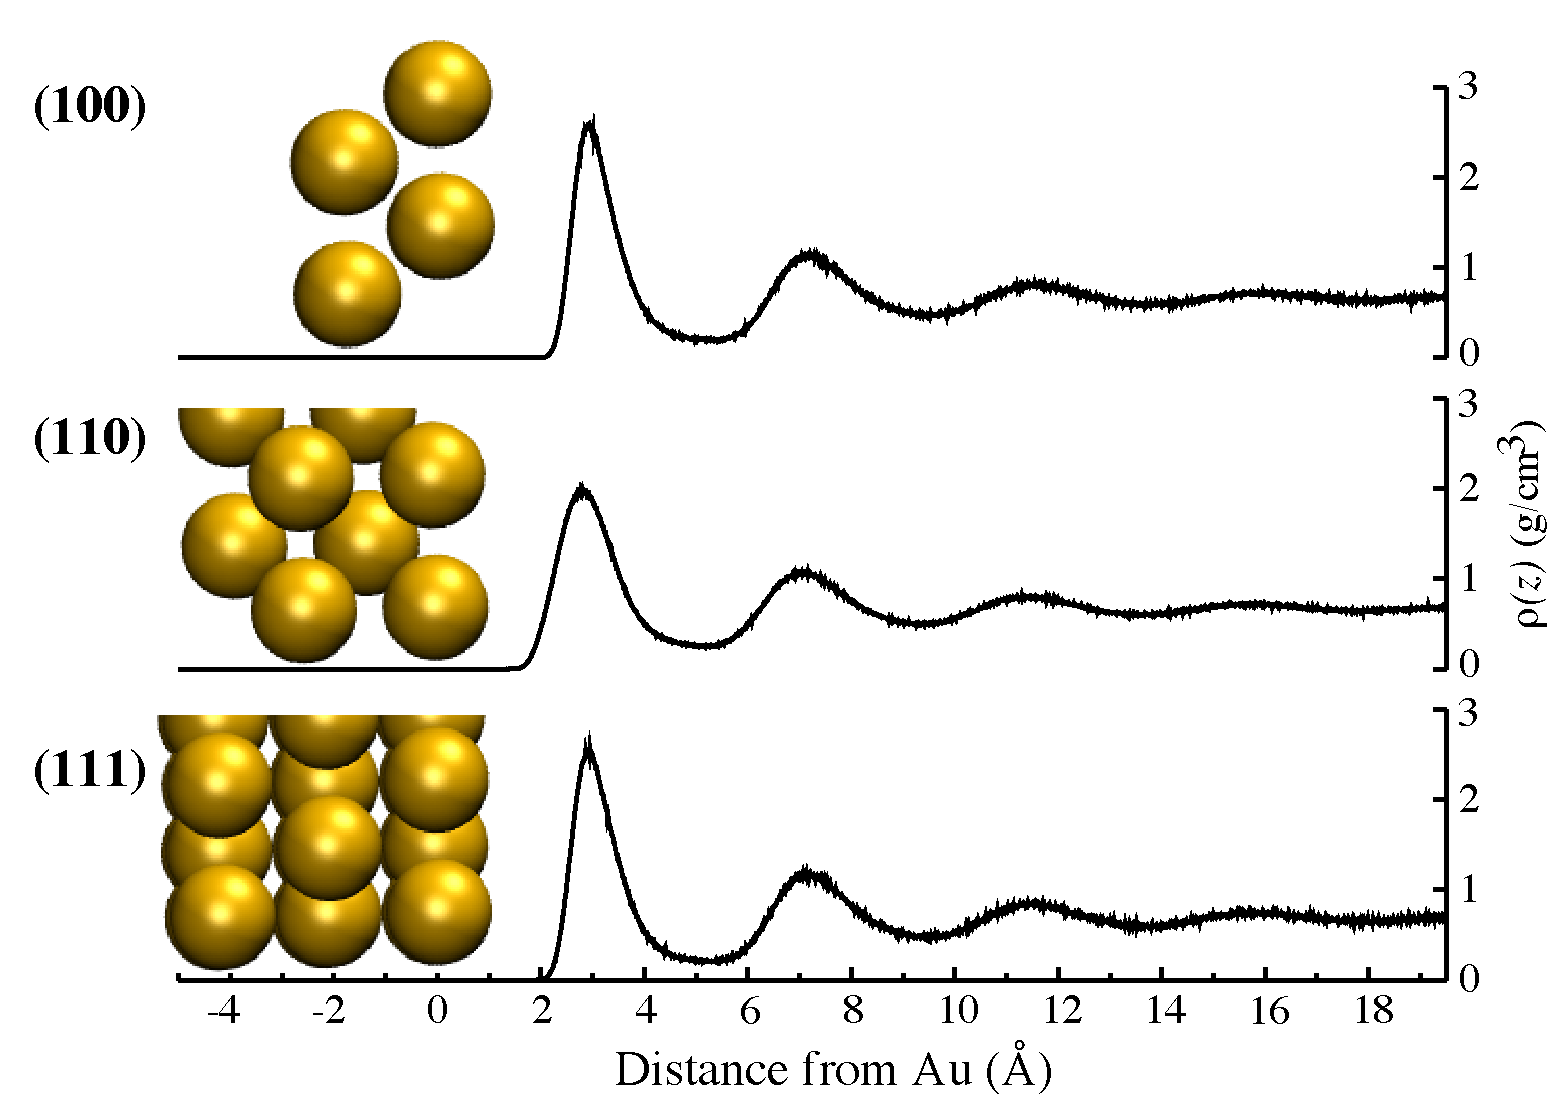
\includegraphics[width=\linewidth]{figures/stacked-hex-facets.pdf}
        \caption{Hexane density as a function of distance from the
          interfacial gold for the (111), (110), and (100) facets. The
          solvent in the (111) and (100) systems display nearly
          identical density profiles. Because the lowest-coordinated
          gold atoms on the (110) facet have a relatively low surface
          density, the hexane molecules are able to get closer to
          these undercoordinated atoms.}
        \label{fig:dens}
\end{figure}

\subsubsection{Surface Atom Undercoordination}
For the three flat facets, the primary feature that differentiates the
facets is the coordination number (CN) of the atoms that are exposed
to the solvent. In bulk Au, the coordination number of the atoms is
twelve; six neighbors in plane, three below the atom, and three above the
atom. Any atom with a coordination number below twelve would exhibit more
vibrational freedom and is considered an undercoordinated site. The
Au(111) surface presents gold atoms with nine surrounding metallic
atoms ($\text{CN} = 9$) to the solvent, while the Au(100) facet
surface exposes atoms with $\text{CN}=8$.  Au(110) displays a
corrugated surface where the two outer layers of atoms have
$\text{CN}=7$ and $\text{CN}=11$, respectively (displayed in \ref{fig:facets-cn}).
Both of the (110) surface atoms coordination environments
approach the surface close enough to interact with the solvent atoms.

\begin{table}
\centering
\caption{Surface densities $(\text{\AA}^{-2})$ of undercoordinated
  atoms in ideal geometries. $\ell~(\text{\AA})$ is the
  lattice constant of the underlying FCC lattice.  The spheres and
  cuboctahedra are calculated using a gold FCC lattice with $\ell = 4.08
  \text{~\AA}$.  For cuboctahedral particles, the radius ($r$) is computed
  using Eq. \eqref{r_ave}.
  \label{tab:undercoord}}
\begin{tabular}{ c|cccc }
\toprule
\multirow{2}{*}{surface} & \multicolumn{4}{c}{Coordination Number}\\
        & 6 & 7 & 8 & 9 \\
 \midrule
(111)      & 0 & 0     & 0     & $\frac{4 \sqrt{3}}{3 \ell^2}$ \\
(100)      & 0 & 0     & $\frac{2}{\ell^2}$ & 0     \\
(110)      & 0 & $\frac{\sqrt{2}}{\ell^2}$ & 0     & 0     \\
 \midrule
Spheres (large $r$ limit)    & 0.021 & 0.025 & 0.021 & 0.032\\ \\
Icosahedra ($n$ shells)  & $\frac{8\sqrt{3}}{5\ell^2n^2}$  &  0 &
 $\frac{4\sqrt{3}(n-1)}{\ell^2n^2}$ &
 $\frac{4(n - 1)}{\sqrt{3}\ell^2 n}$ \\ \\
Cuboctahedra & 0 & $\frac{1}{r\ell} \left(\frac{3\sqrt{2} + 2\sqrt{6}}{3+\sqrt{3}}\right)$ & $\frac{6}{(3+\sqrt{3})\ell^2}$ & $\frac{4}{(3+\sqrt{3})\ell^2}$\\ \\
\bottomrule
\end{tabular}
\end{table}

In Table \ref{tab:undercoord}, the surface density of
undercoordinated atoms for a set of ideal geometries are provided.
The population
density for the sphere systems in the large radius limit are taken by
averaging the surface densities for ideal gold nanospheres with radii
of 95--100 \AA.  For other FCC-based nanoparticles, it is relatively
simple to convert these surface densities using the lattice constant
of gold, $\ell = 4.08 \text{~\AA}$.

Planar facets have a fixed population density based on the number of
exposed undercoordinated atoms and the physical dimensions of the
exposed facet area in terms of the lattice constant.
\begin{figure}[!htb]
        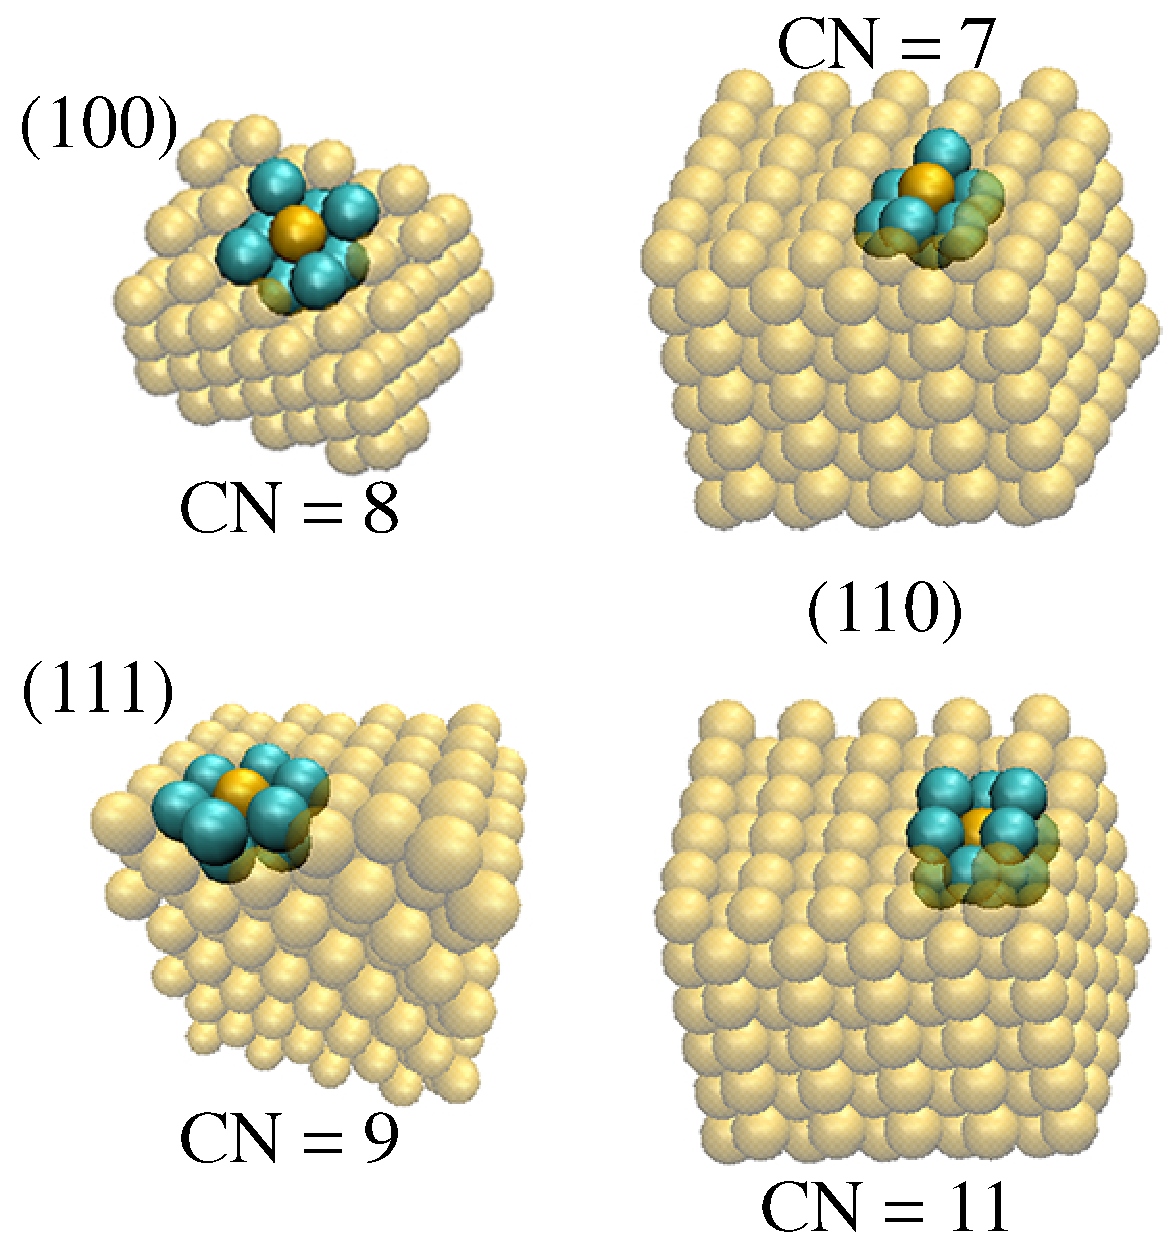
\includegraphics[width=5in]{figures/facets-cn.pdf}
        \caption{Locations of undercoordinated atoms on common gold
          facets. The dark gold atoms indicate atoms of a particular
          coordination number, cyan atoms denote the first nearest
          neighbors of these atoms, and the partially transparent
          lattice illustrates the location of the atoms in the larger
          gold structure. (111) surfaces (lower left) display atoms
          with CN=9, while (100) surfaces (upper left) display atoms
          with CN=8, and (110) surfaces present surface atoms with
          CN=7 and buried atoms with CN=11. }
        \label{fig:facets-cn}
\end{figure}
In an ideal icosahedral nanoparticle with $n$ shells, the surface
population density is computed using the number of vertex, edge, and
face atoms,
\begin{align}
n_\text{vertex} & = 12, \\
n_\text{edge} & = 30 (n -1), \\
n_\text{face} & = 10 n^2 - 30 n + 20.
\end{align}
The number of shells, $n$, is also directly related to the particle
edge length ($a$), radius ($r$), and surface area ($A$) of the
icosahedral particle,
\begin{align}
a & = \ell~n \\
r & = \frac{\ell~n~\sqrt{10+2\sqrt{5}}}{4} \\
A & =  \ell^2~n^2~ 5 \sqrt{3}
\end{align}
where $\ell$ is the lattice constant.

For ideal cuboctahedra, the edge length ($a$) can be used to determine
surface areas for the eight triangular (111) faces and six square
(100) faces,
\begin{align}
A_\mathrm{(111)} &= 2 \sqrt{3} a^2 \\
A_\mathrm{(100)} &= 6 a^2
\end{align}
In addition, cuboctahedra have twenty-four edges (CN = 7, length =
$a$), and twelve vertices (CN = 5).  An approximate radius of the
cuboctahedral particles can be found by averaging the diameter between
parallel square faces and parallel triangular faces,
\begin{equation}
r  = \frac{a}{2} \left(\frac{\sqrt{2}}{2} + \frac{\sqrt{6}}{3}\right)
\label{r_ave}
\end{equation}
Table \ref{tab:undercoord}.  Surface densities of the CN=9 and CN=8
sites are computed using the fraction of total surface area in each of
the (111) and (100) facets, respectively.  For small particles, the
edge atoms (CN=7) can dominate, but for larger particles, the ratio of
CN=8 and CN=9 atoms is constant.



% \begin{figure}
% 	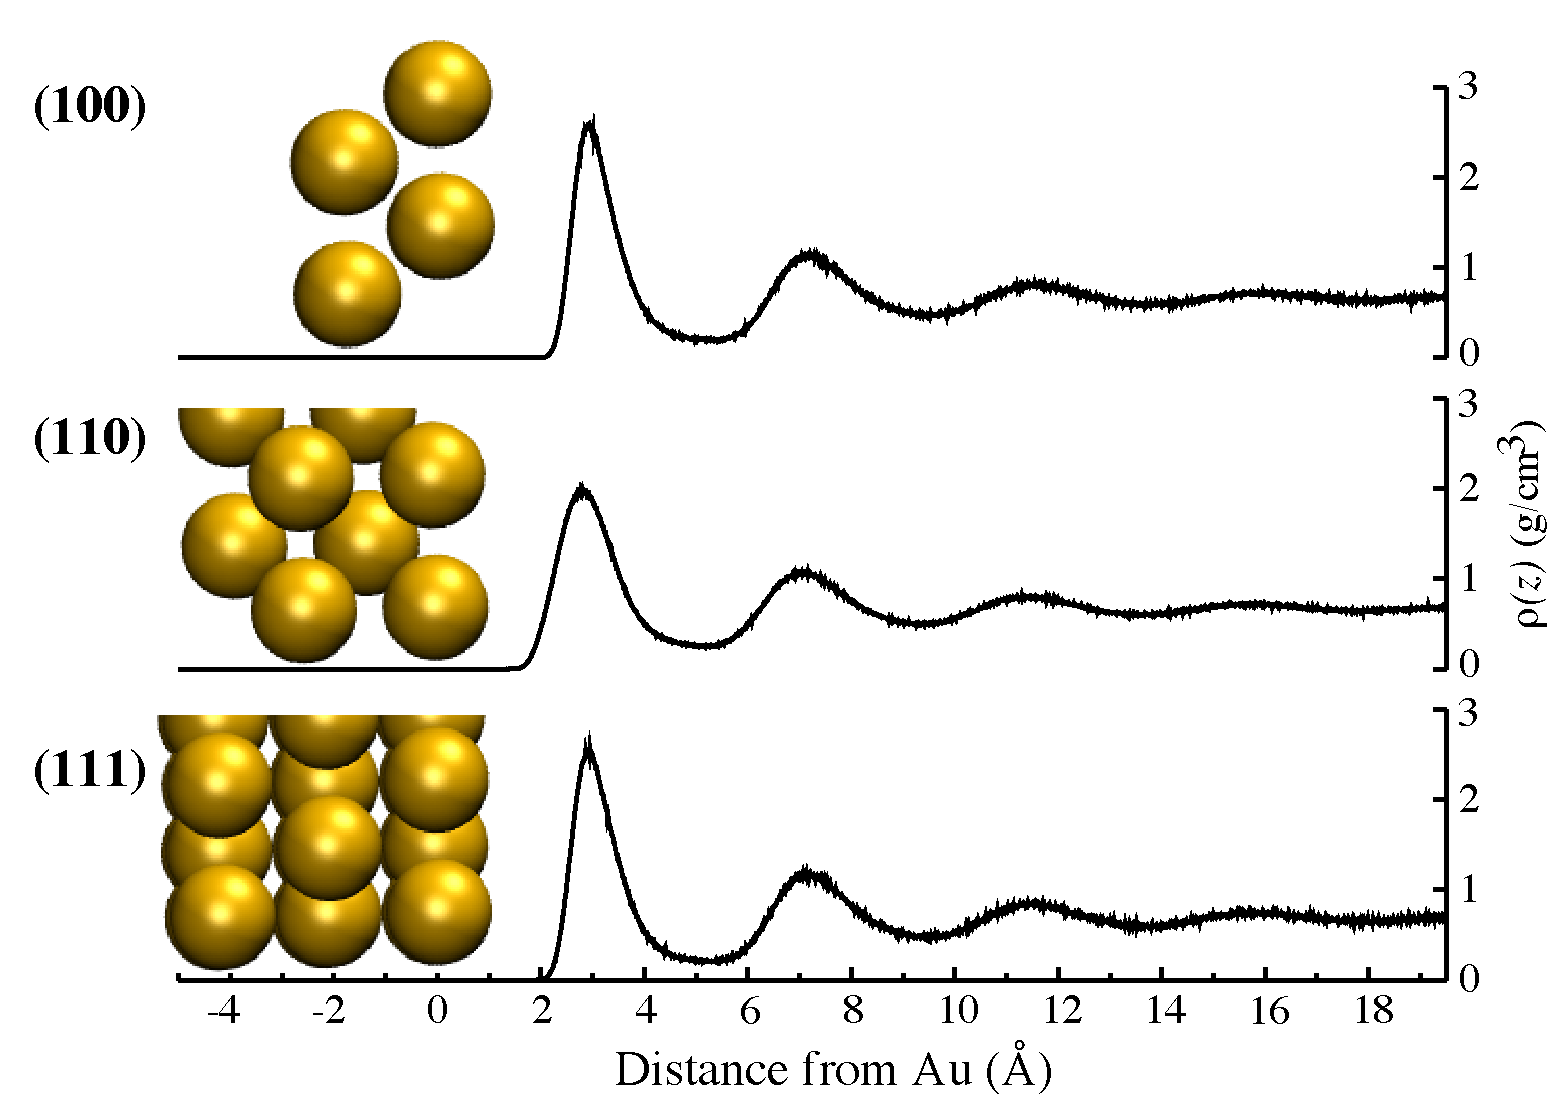
\includegraphics[width=\linewidth]{figures/stacked-hex-facets.pdf}
% 	\caption{The hexane density as a function of distance from the interfacial gold for the (111), (110), and (100) facets. The solvent in the (111) and (100) systems display nearly identical density profiles. Because the lowest-coordinated gold atoms on the (110) facet have a relatively low surface density, the hexane molecules are able to get closer to these undercoordinated atoms.}
% 	\label{fig:dens}
% \end{figure}

Reducing the number of metallic interactions allows the surface atoms
to vibrate at different frequencies than the interior atoms,
populating a portion of the spectrum that overlaps with collective
motions of the solvent molecules. This mechanism may explain the
enhanced interfacial thermal conductance of the (100) facet relative
to the (111) facet. However, it does not explain why the (110) facet
displays an intermediate conductance even though the surface atoms
have a lower coordination number than the (100) facet.  To answer this
question, it is important to consider the surface density of the
undercoordinated atoms as well as the vibrational freedom allowed by
the undercoordination. In Table \ref{tab:au-den} the density
of the solvent-accessible undercoordinated surface atoms for the three
facets is shown. Although the (110) facet displays 7- and 11-coordinated atoms
to the solvent, the $\text{CN}=11$ have vibrational dynamics that are
essentially equivalent to the bulk gold (Fig. \ref{fig:cn-spect}), and the
surface density of these atoms is significantly lower than the surface
density displayed by the (111) and (100) facets.

\begin{figure}[!htb]
  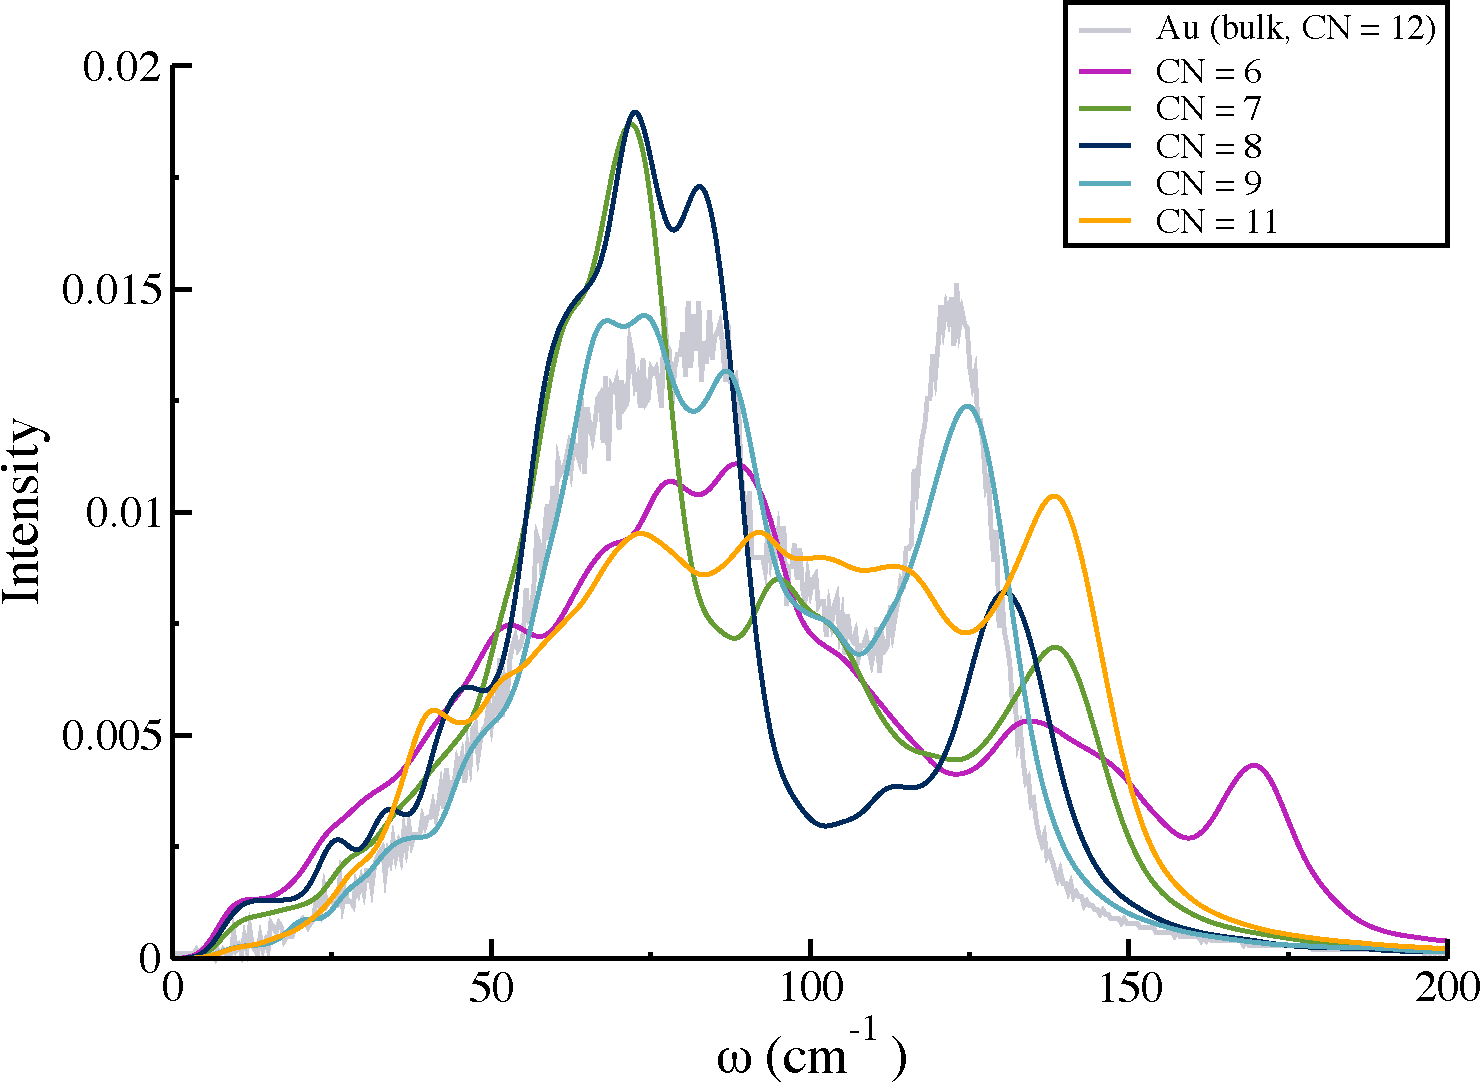
\includegraphics[width=5in]{figures/surface-cn.pdf}
  \caption{The normalized low frequency density of states (DOS) of the
    surface atoms with the coordination number of 6, 7, 8, 9 and 11,
    corresponding to the vertices of the icosahedra, Au(110), Au(100),
    Au(111) and subsurface Au(110), respectively.  Note that CN=11
    atoms near a surface are found adjacent to atoms with lower
    coordination (e.g. CN=7), so the high frequency peak at 138
    cm$^{-1}$ is present for both CN=11 and CN=7.  Low frequency
    contributions at $\sim$ 70 cm$^{-1}$ are enhanced for surface
    atoms with CN=7, 8, and 9.}
  \label{fig:cn-spect}
\end{figure}

\begin{table}[h]
\centering
\caption{The density of undercoordinated gold atoms at the surface of a facet.  
\label{tab:au-den}}
\renewcommand*{\arraystretch}{2}
\begin{tabular}{ ccc }
\toprule
Facet & CN & Surface Density (atoms $\text{\AA}^{-2}$)\\
\midrule
        (111) & 9  & 0.1394 \\
\midrule
        (100) & 8  & 0.1214 \\
\midrule
        (110) & 7  & 0.0877 \\
              & 11 & 0.0877 \\
\bottomrule
\end{tabular}
\end{table}

It is therefore likely that not only the undercoordination of surface
atoms, but also the density of these undercoordinated atoms plays a
role in thermal conductance. In the nanoparticles, surface atoms that
are in physical contact with the solvent have a range of coordination
numbers from $5 - 9$, but only $\text{CN} = 6 - 9$ appear with high
probability.  The surface coordination densities have been calculated
for all of our samples, and the undercoordination density is distinct
for the spheres, icosahedra, and cuboctahedra (See
Fig. \ref{fig:stacked-cn}).

The icosahedral particles display three coordination environments: the
vertices have a $\text{CN} = 6$, while the triangular (111) faces of
the particle have a $\text{CN} = 9$, and the edges connecting the
faces have $\text{CN} = 8$.  As the radius of the icosahedral
particles increases, the surface is dominated by the triangular
facets, so the surface density of the $\text{CN} = 9$ rises.  For
perfect icosahedra, the ideal surface densities are shown as dashed
lines in Fig. \ref{fig:stacked-cn}.

For the simulated systems at 250K, surface vibrational motion leads to
coordination numbers that are lower than one would expect for an ideal
icosahedron. This is evident in the populations of the $\text{CN}= 9$,
which is 20-50\% lower than the ideal case.

\begin{figure}
	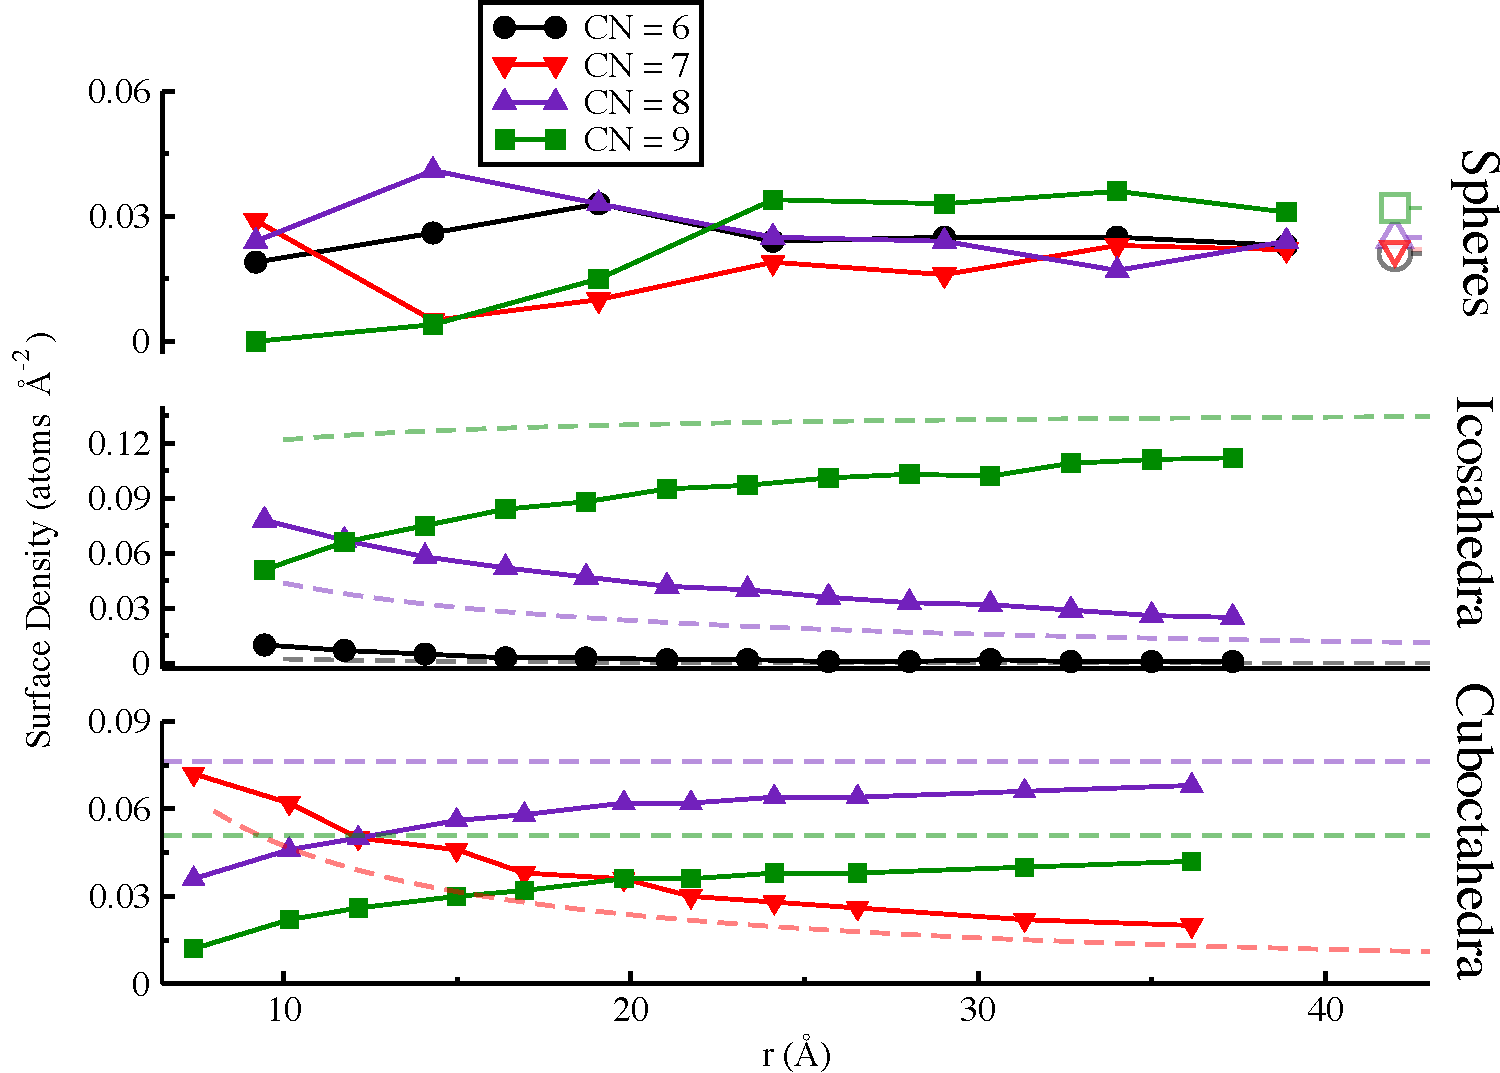
\includegraphics[width=\linewidth]{figures/new-cn.pdf}
	\caption{The coordination number of surface atoms as a
          function of particle size. Filled data points are sampled
          from simulations, while the dashed lines correspond to ideal
          icosahedral and cuboctahedral solids. In the spherical case,
          the large radius limits are shown with open symbols.  The
          large radius limit for the spheres approaches a constant
          density for all undercoordinated sites, while for the
          icosahedra, the 9-coordinated (111) facet dominates. In
          larger cuboctahedra, the relative fraction of 8- and
          9-coordinated surface atoms is largely independent of
          particle size.} 
	\label{fig:stacked-cn}
\end{figure}

In the spherical particles, the surface density of undercoordinated
atoms stabilizes above $r = 25$ \AA.  However, the densities of the
undercoordinated atoms never approach any of the flat facet values (as
is the case in the icosahedra).  We may estimate the large radius
limit of the spheres by averaging the surface densities for ideal
spheres of radii 95--100 \AA.  These are shown with open symbols in
the upper panel of Fig. \ref{fig:stacked-cn}.

The cuboctahedral particles approach the ideal solid surface densities
as the radius of the particle increases. Beyond a radius of 15 \AA\,
the cuboctahedra are no longer dominated by edge atoms and flat facets
form the majority of the surface. After this transition the surface
densities quickly stabilize to nearly-ideal cuboctahedral structures.

\subsubsection{Phonon Spectra}
By selecting specific groups of atoms while computing the vibrational
power spectrum (Eq. \ref{eq:DOS}) the role of
undercoordination on surface vibrational motion can be explored. For thermal
transport, the regions of interest are the nanoparticle atoms in
direct physical contact with the solvent, and those solvent molecules
that form the first solvation shell, i.e. $< 5 \text{\AA}$ from the
gold surface.

Under the QSC potential, the bulk gold vibrational power spectrum
displays two broad peaks, one at $\sim 60-80 \text{~cm}^{-1}$, and
another sharper peak at $\sim 125 \text{~cm}^{-1}$.  The vibrational
densities of states for the four outer layers of the nanoparticles are
shown in Fig. \ref{fig:layer}.  The surface layers for all particles
are dominated by the low frequency portion of the spectrum
($<70 \text{~cm}^{-1}$) and display small morphology-dependent
features at higher frequencies ($140 \text{~cm}^{-1}$). The
low-frequency peak appears at significantly lower frequencies than in
the bulk, and the higher frequency contribution is significantly
broadened.  Spheres and cuboctahedra recover bulk-like densities of
states relatively close to the surface -- only the surface and second
shell are significantly altered from the bulk gold density of
states. In the spheres, the higher frequency contribution
($\sim 150 \text{~cm}^{-1}$) resembles the vibrational density of
states for undercoordinated atoms with CN=8 or 7 (see 
Fig. \ref{fig:cn-spect}).

\subsubsubsection{A Brief Aside}
The icosahedra still have perturbed spectra even four layers into the
particles. Icosahedral particles grow around a core with
$\mathrm{I}_h$ symmetry, and the local environment around the atoms
deviates significantly from perfect FCC ordering.  The local bond
orientational order can be described using the method of Steinhardt
\textit{et al.}\cite{Steinhardt1983} 
The local bonding environment,
$\bar{q}_{\ell m}$, for each atom in the system is determined by
averaging over the spherical harmonics between that atom and each of
its neighbors,
\begin{equation}
\bar{q}_{\ell m} = \sum_i Y_\ell^m(\theta_i, \phi_i)
\end{equation}
where $\theta_i$ and $\phi_i$ are the relative angular coordinates of
neighbor $i$ in the laboratory frame.  A global average orientational
bond order parameter, $\bar{Q}_{\ell m}$, is the average over each
$\bar{q}_{\ell m}$ for all atoms in the system. To remove the
dependence on the laboratory coordinate frame, the third order
rotationally invariant combination of $\bar{Q}_{\ell m}$,
$\hat{w}_\ell$, is utilized here.\cite{Steinhardt1983,Vardeman:2008fk}

For $\ell=4$, the ideal face-centered cubic (FCC) local structures
exhibit $\hat{w}_4$ values near -0.159. Because $\hat{w}_4$ exhibits
an extreme value for fcc structures, it is ideal for measuring local
FCC ordering. The spatial distribution of $\hat{w}_4$ local bond
orientational order parameters, $p(\hat{w}_4 , r)$, can provide
information about the location of individual atoms that are central to
local FCC ordering.

The fraction of FCC-ordered gold atoms at a given radius in the
nanoparticle,
\begin{equation}
        f_\mathrm{fcc}(r) = \int_{-\infty}^{w_c} p(\hat{w}_4, r) d \hat{w}_4
\end{equation}
is described by the distribution of the local bond orientational order
parameters, $p(\hat{w}_4, r)$, and $w_c$, a cutoff for the peak
$\hat{w}_4$ value displayed by fcc structures. As in our previous
work,\cite{Stocker2016} $w_c$ value of -0.12 was chosen to isolate the
fcc peak in $\hat{w}_4$.

As shown in Fig. \ref{fig:struct-bowr}, the FCC ordering persists in
the spheres even quite close to the surface, while the icosahedra have
significant populations that deviate from FCC local ordering.  The
cuboctahedra do not have uniform gold population between 30 and 40
\AA, so the fraction of FCC ordering decays starting at 30 \AA.
Although I cannot conclude that this is the cause of the differences
in the VDOS for the icosahedral particles, it is likely that local
ordering in the metal can alter the bulk densities of states.

\begin{figure}[!htb]
        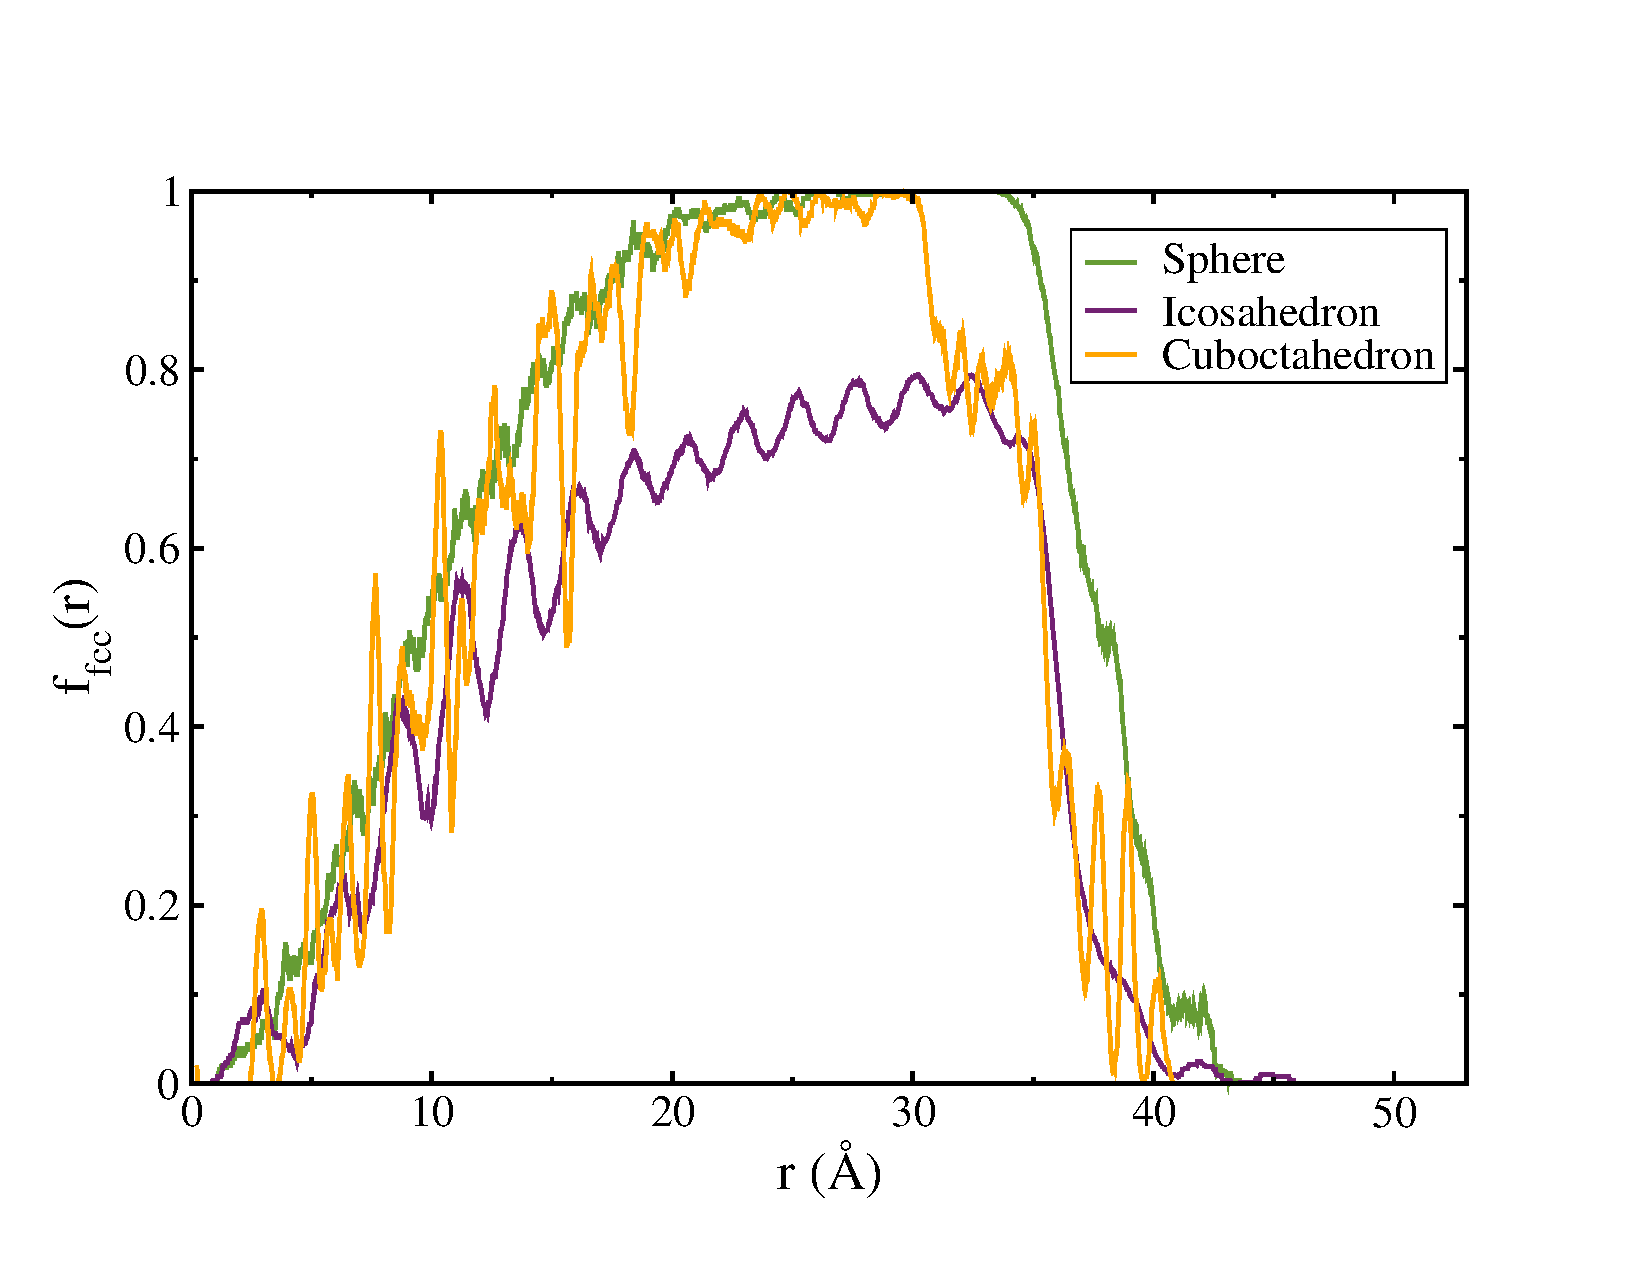
\includegraphics[width=5in]{figures/struct-bowr.pdf}
        \caption{The fraction of FCC-like local environments as a
          function of radius from the center of 40 \AA\ nanoparticles.
          The spheres and cuboctahedra are originally cut from a FCC
          lattice, so the local ordering persists even close to the
          surface.  Icosahedra are constructed as shells surrounding a
          perfectly icosahedral central core of 13 atoms. Non-FCC
          ordering persists throughout these simulations.}
        \label{fig:struct-bowr}
 \end{figure}

%The icosahedra therefore display phonon
%spectra that are enhanced in the higher frequency peaks
%($\sim 130 \text{~cm}^{-1}$) at the expense of the broad
%$\sim 60-80 \text{~cm}^{-1}$ feature.

\begin{figure}
	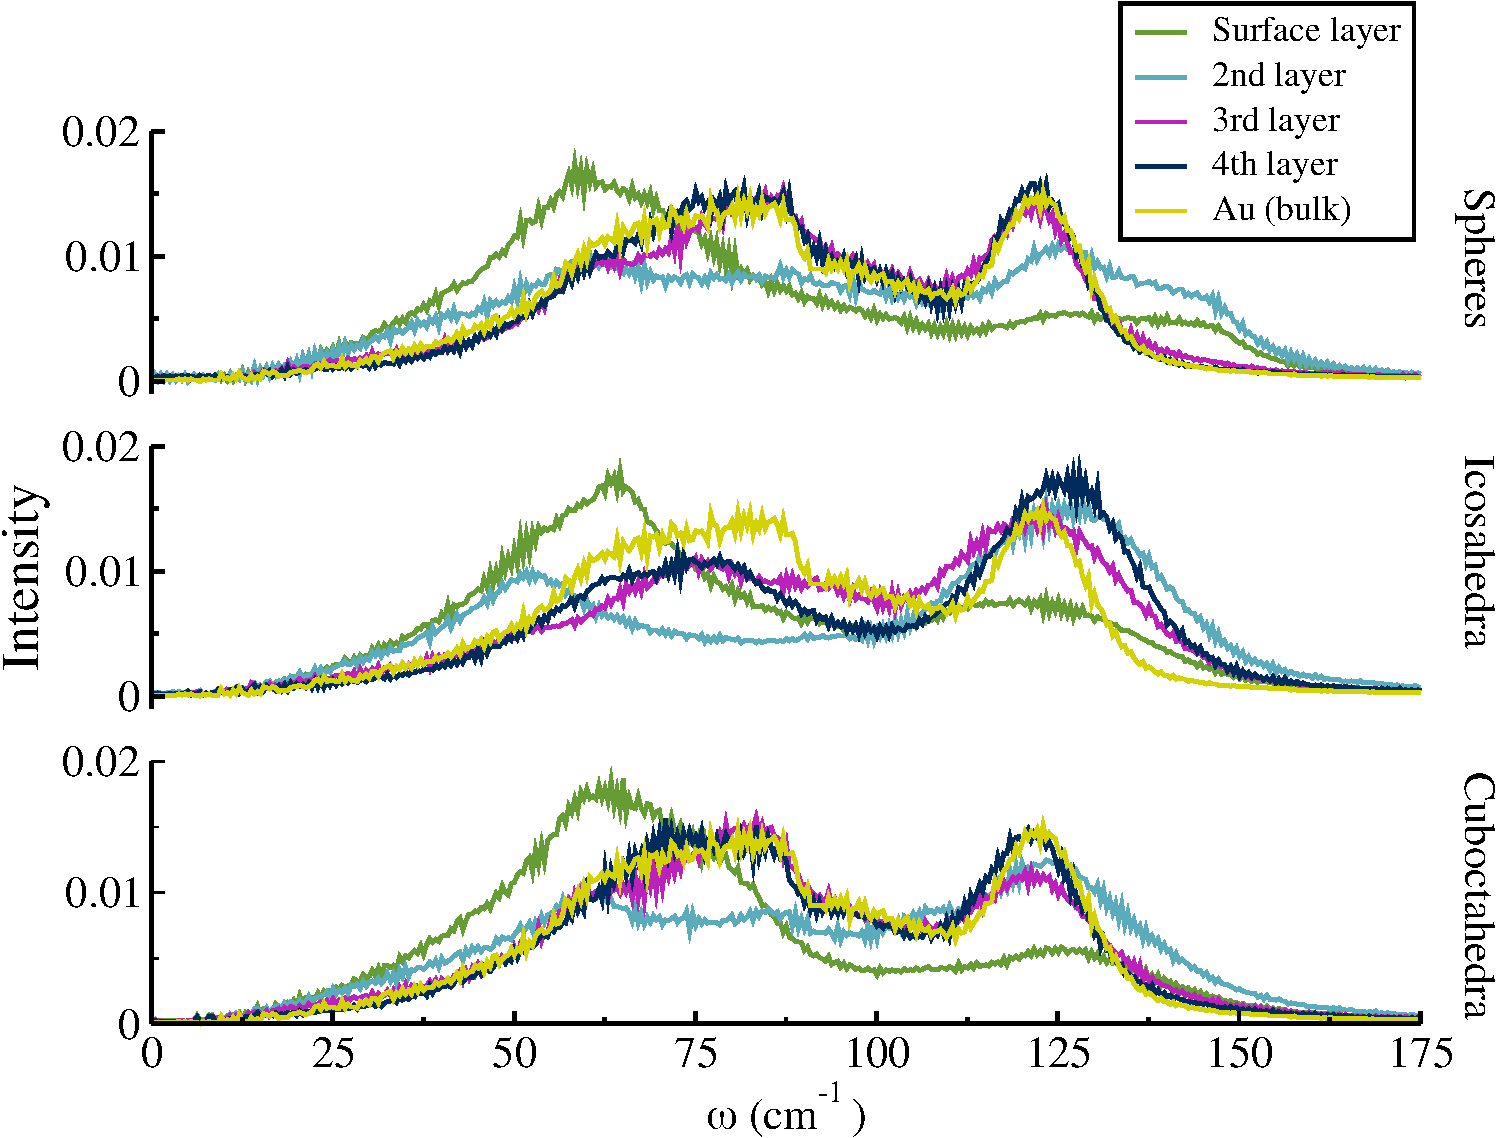
\includegraphics[width=\linewidth]{figures/col-layer40.pdf}
	\caption{The projected vibrational density of states
          (Eq. \ref{eq:DOS}) for individual layers in the largest gold
          nanoparticles (top: spheres, middle: icosahedra, bottom:
          cuboctahedra). In all systems, the surface layer (green) is
          significantly enhanced at low frequencies and is shifted
          down by $\sim~20\text{~cm}^{-1}$. The Au (bulk) curve shown
          for comparison is from a perfect FCC lattice in periodic
          boundary conditions.}
	\label{fig:layer}
\end{figure}

Comparison of the vibrational density of states of all the gold atoms
displays some important differences between the icosahedral structures
and the FCC-based spheres and cuboctahedra
(Fig. \ref{fig:all-v-surf}).  Icosahedral particles have non-FCC
ordering deep into the particle, and this manifests as a shift in
phonon population from the broad low-frequency region to the higher
frequency peak, even for the largest of the particles that were
studied.  For comparison, the largest spheres and icosahedra have only
slight differences in their ``bulk'' phonon density of states.

At the surfaces of the particles, the differences are nearly all in
the higher frequency portion of the spectrum ($>100 \text{cm}^{-1}$),
indicating that the surface undercoordination primarily alters
high-frequency transmission into the solvent.  This suggests roles for
bulk crystalline ordering as well as surface undercoordination in any
model for the interfacial thermal conductance.

\begin{figure}
	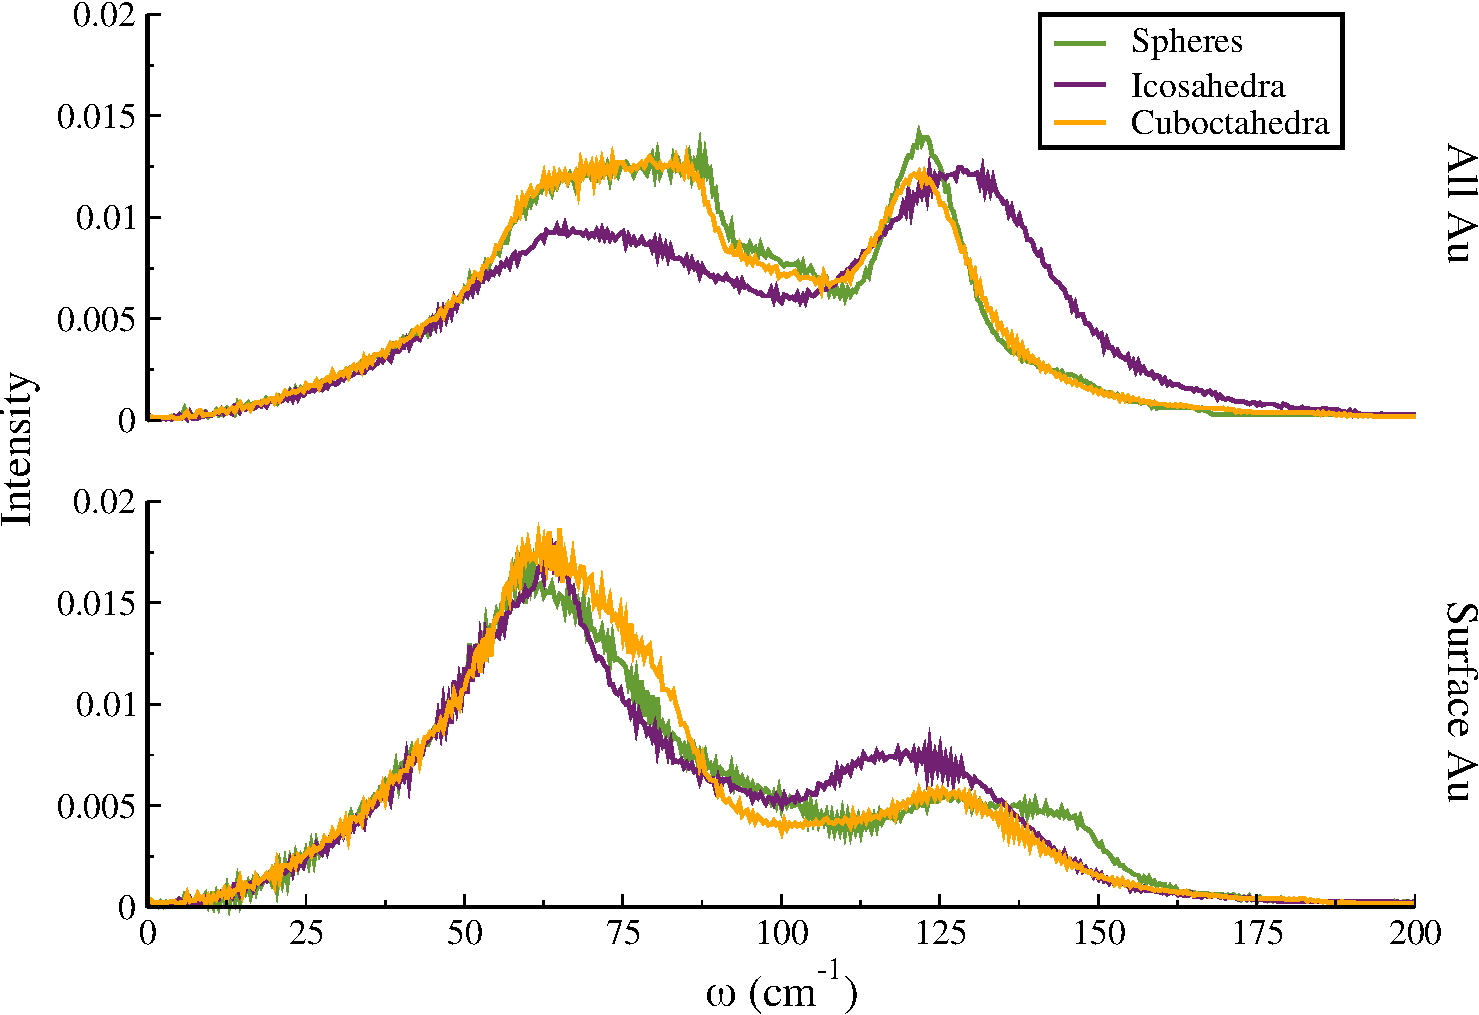
\includegraphics[width=\linewidth]{figures/all-v-surface.pdf}
	\caption{The projected vibrational density of states for all
          gold atoms (top panel) shows that the phonons in FCC-like
          nanoparticles (spheres, cuboctahedra) have similar frequency
          representation, while the non-FCC structures (icosahedra)
          have significantly altered ``bulk'' spectra. For surface
          atoms (bottom panel), the differences in surface
          undercoordination  appear at higher frequencies.  These
          spectra were computed for the largest particles in each of
          the different morphologies.}
	\label{fig:all-v-surf}
\end{figure}

Except in the case of the icosahedra, vibrational power spectra that
include all gold atoms in the nanoparticles do not show significant
dependence on particle radius (see Fig. \ref{fig:all-spect}.  This
suggests that mismatch models (like AMM or DMM) that use only bulk
properties will not be able to capture the surface behavior that is
relevant to heat transfer at the nanoscale.

%Projecting out the phonon contributions that are normal to the interface and assuming that phonon group velocity is always tied to the bulk speed of sound leads us to a relatively simple phonon transmission model,
% \begin{equation}
% \tau_{a \rightarrow b}(\omega) = \frac{v_b \rho^\perp_b(\omega)}{v_a \rho^\perp_a(\omega) + v_b \rho^\perp_b(\omega)}
% \label{eq:transmission}
% \end{equation}
% where $v_a$ and $v_b$ are the speeds of sound in the two materials.  We have used $v_\text{Au} = 3240 \text{~m s}^{-1}$ and $v_\text{hexane} = 1122 \text{~m s}^{-1}$ for hexane at similar conditions.\cite{CRC,Ball2001}  $\rho^\perp(\omega)$ is the projected density of states, and we are suggesting that the density of states should include only the atoms at the interface that are in \textit{direct physical contact}, i.e. the surface layer of gold atoms and hexane within 5 \AA\ of the gold particle. 

% The frequency-dependent transmission probabilities computed using these assumptions are shown in Fig. \ref{fig:transmission}. The most important differences appear in the heat-carrying modes below $50 \text{~cm}^{-1}$. For the spherical particles, the transmission probabilities in the low frequency region show the same trend as the thermal conductance ($G$) values.  The low-frequency phonon transmission probabilities increase with particle radius until the particles reach $\sim 20 \text{~\AA}$.  Above this size, transmission in this range has converged to the large particle behavior.  

% The icosahedral particles exhibit much more uniform behavior under this transmission model, with variations only for the smallest particles.  A reasonable explanation for this observation is that the surface layers are dominated by the $\text{CN} = 9$ atoms, which all have similar contributions to the vibrational density of states.

% \begin{figure}
% 	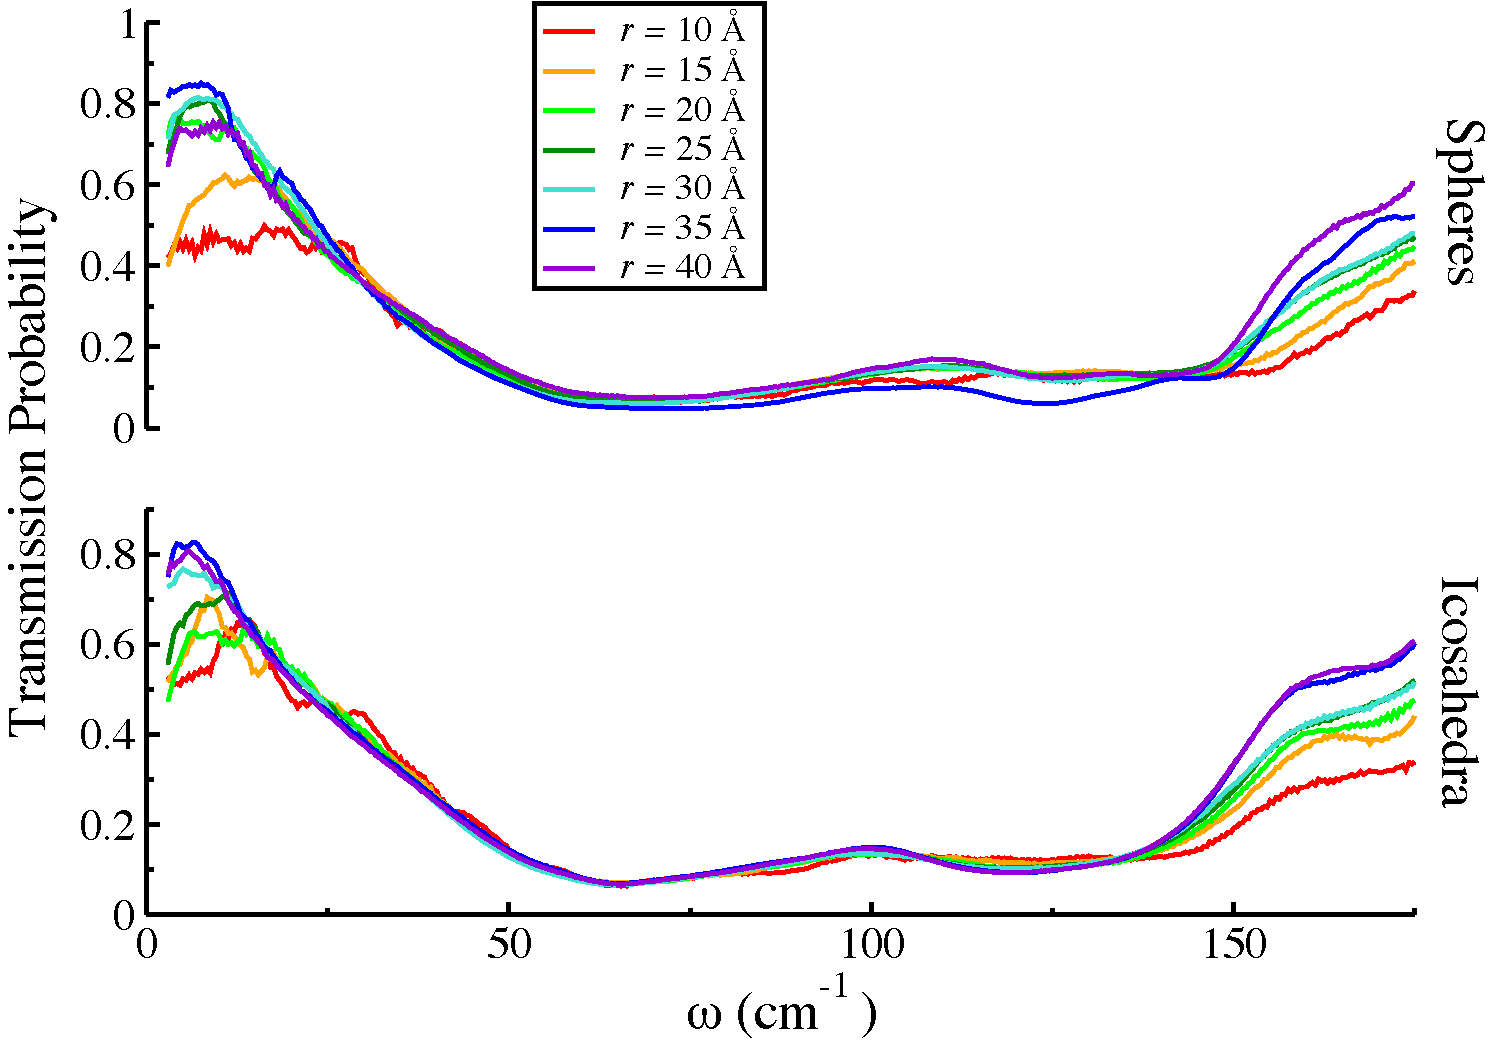
\includegraphics[width=\linewidth]{figures/col-transmission.pdf}
% 	\caption{The frequency-dependent phonon transmission model, Eq. (\ref{eq:transmission}), predicts size-dependent phonon transmission at lower frequencies ($< 50 \mathrm{~cm}^{-1}$), and this effect is particularly pronounced in the spherical nanoparticles.  Icosahedral surfaces are dominated by the $\text{CN} = 9$ atoms, so differences in the low-frequency transmission are diminished.}
% 	\label{fig:transmission}
% \end{figure}

Solvent vibrational densities of states are remarkably similar for the
icosahedral and spherical particles, even for solvent that is within 5
\AA\ of the interface (Fig. \ref{fig:all-spect}). 
While the solvent VDOS in the icosahedral
and spherical systems shows only small changes as a function of
particle size, the solvent in the cuboctahedral systems appears to
shift to lower frequencies with increasing particle radius.  The gold
VDOS in all systems displays a shift from the low frequency peak,
$70 \mathrm{~cm}^{-1}$, to a peak at $125 \mathrm{~cm}^{-1}$ as the
particle radii increases and there is a significant difference between
the two FCC structures and the icosahedra spectra.  The FCC structures
increase in intensity at $125 \mathrm{~cm}^{-1}$ with increasing
particle radius, while the icosahedra VDOS shows a shift in population
from low frequencies to the higher frequency peak.  Note that the gold
shown in Fig. \ref{fig:all-spect} includes all layers of the
particles.

Due to the similarity in solvent VDOS, a model for interfacial 
thermal transport in these
systems would need to include the lattice structure of the particle
and the quantity and solvent accessibility of specific kinds of
undercoordinated metal atoms.

\begin{figure}[!htb]
        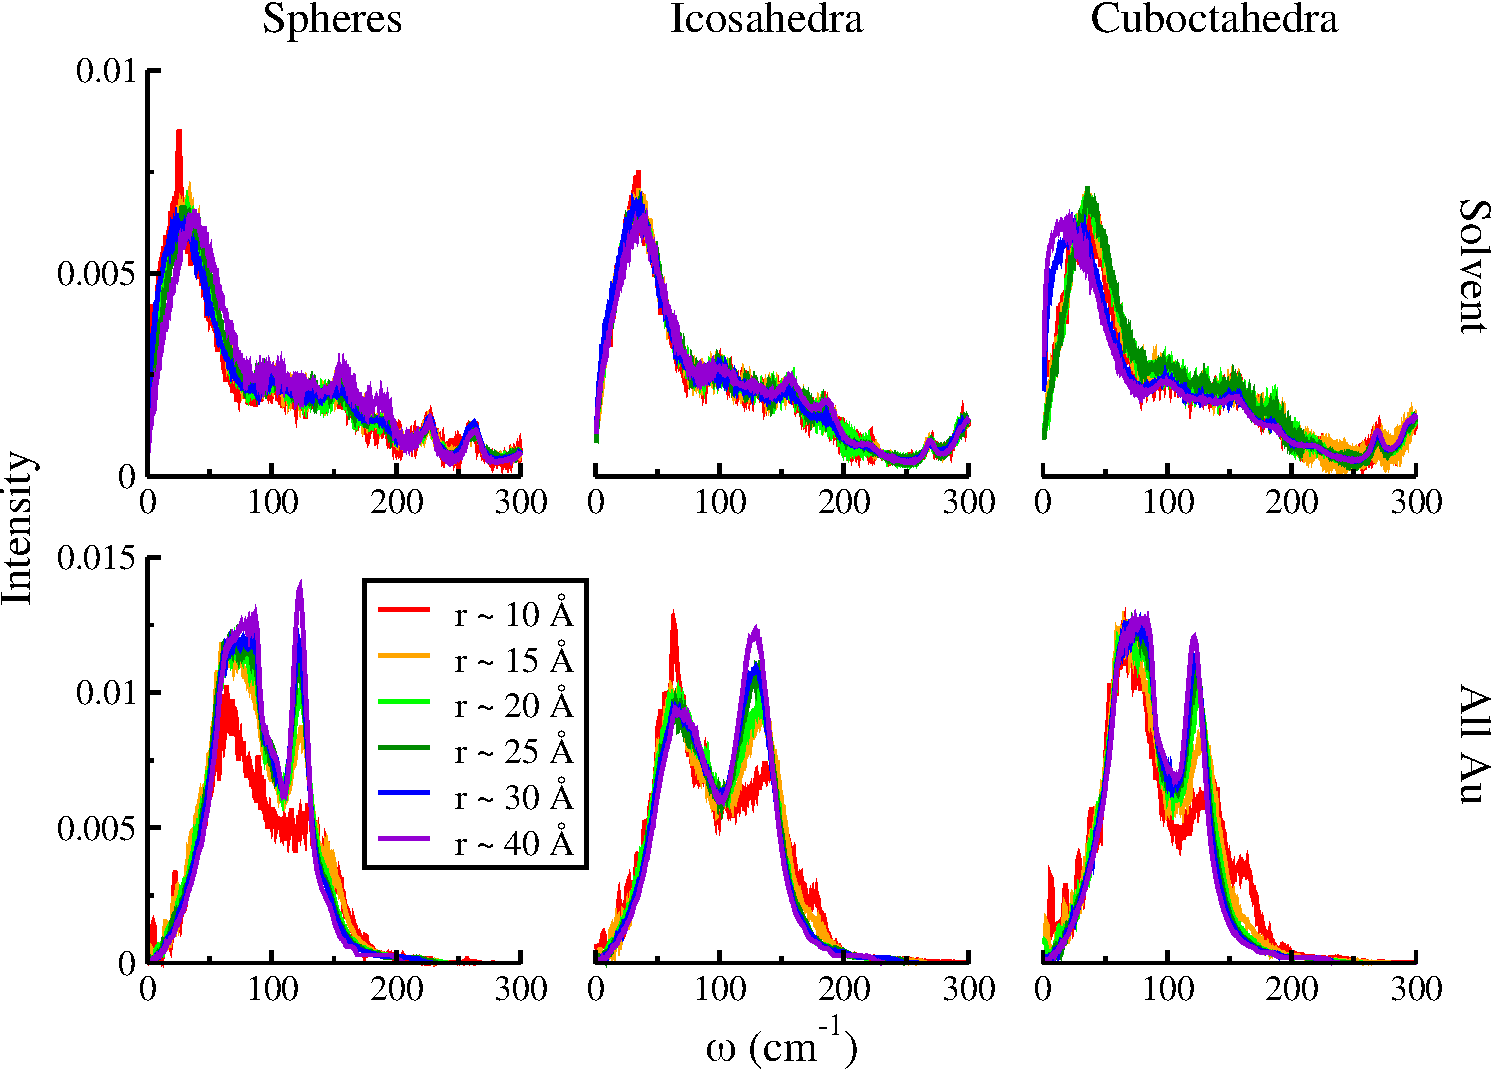
\includegraphics[width=5in]{figures/all-spect.pdf}
        \caption{The normalized low frequency density of states (DOS)
          of the interfacial solvent and the gold particle for the
          icosahedral and spherical systems. }
        \label{fig:all-spect}
\end{figure}

\subsubsection{A Simple Model for Bare Nanoparticle Conductance}
The vibrational densities of states suggest the bare metallic
nanoparticles exhibit different bulk phonon frequencies that depend on
crystalline packing, and different surface spectra that depend on
surface undercoordination.  Both of the bulk and surface frequencies
can effect thermal transport, so a simple model in terms of a linear 
combination of surface densities of undercoordinated atoms can be explored,
\begin{equation}
G \approx a~\mathrm{CN}_{6} + b~\mathrm{CN}_{7} + c~\left(1+c^{\prime}~\delta_\mathrm{ico}\right)~\mathrm{CN}_{8} + d~\left( 1 + d^{\prime}~\delta_\mathrm{ico} \right)~\mathrm{CN}_{9}
\label{eq:lin-fit}
\end{equation}
where, $a - d$ are coordination transport coefficients with the units
of $10^{-20}$ MW/K and $\mathrm{CN}_{n}$ have surface density units
(1/\AA $^2$) for surface atoms with coordination number $n$.  The
delta function, $\delta_\mathrm{ico}$ is set to unity for icosahedral
structures, and zero for FCC-like nanoparticles.  The coefficients
$c^{\prime}$ and $d^{\prime}$ are weighting factors that recognize the
differences in the bulk density of states in the icosahedral
particles.  Fitting the six parameters was done using a simple
ordinary least squares model with data from all simulated particles.

\begin{table}
\centering
\caption{Parameters of the Model in Eq. (\ref{eq:lin-fit}).
  \label{tab:coeff to fit}}
\begin{tabular}{ cccccc }
\toprule
 $a$ & $b$ & $c$ & $c^{\prime}$ & $d$ & $d^{\prime}$ \\
\midrule
 858.9405 & 183.9062 & 291.7960 & -0.5943 & 369.6250 & -0.2498 \\
\bottomrule
\end{tabular}
\end{table}

With Eq. \eqref{eq:lin-fit} it should be possible to predict the
interfacial thermal conductance for bare gold nanoparticles in hexane
based only on a structural analysis of the surface for coordination
densities and the interior of the particle for crystalline structure.
The predicted (and simulated) values of the thermal conductance are
given in Fig. \ref{fig:models}.  With a coefficient of determination
($R^2$) value of 0.656, this fit does not predict $G$ with a high
degree of certainty, but it does suggest the large role that
undercoordinated surface atoms play in conductance. Coefficients used
in Eq. \eqref{eq:lin-fit} are given in Table \ref{tab:coeff to fit}.

The coefficients provide some information about the thermal transport
capabilities of each type of undercoordinated surface atom. These fits
suggest that severely undercoordinated atoms (CN=6) transfer the
largest amount of heat per atom, although their population in all
systems is low.

It is also important to note that this fit considers the two different
types of particles when finding the best fits for the most populous
surface atoms (CN=8, CN=9).  If the system is FCC-like the weight of
the CN = 8 and CN = 9 are 2.464 and 1.333 times larger than their
contributions from icosahedral cores.

Since the coefficients are related to the amount of energy transfered
per atom type, these atoms on the FCC-like structures transfer a
larger amount than in the icosahedral structure.  This is likely due
to differences in the underlying ``bulk'' densities of states.

\begin{figure}
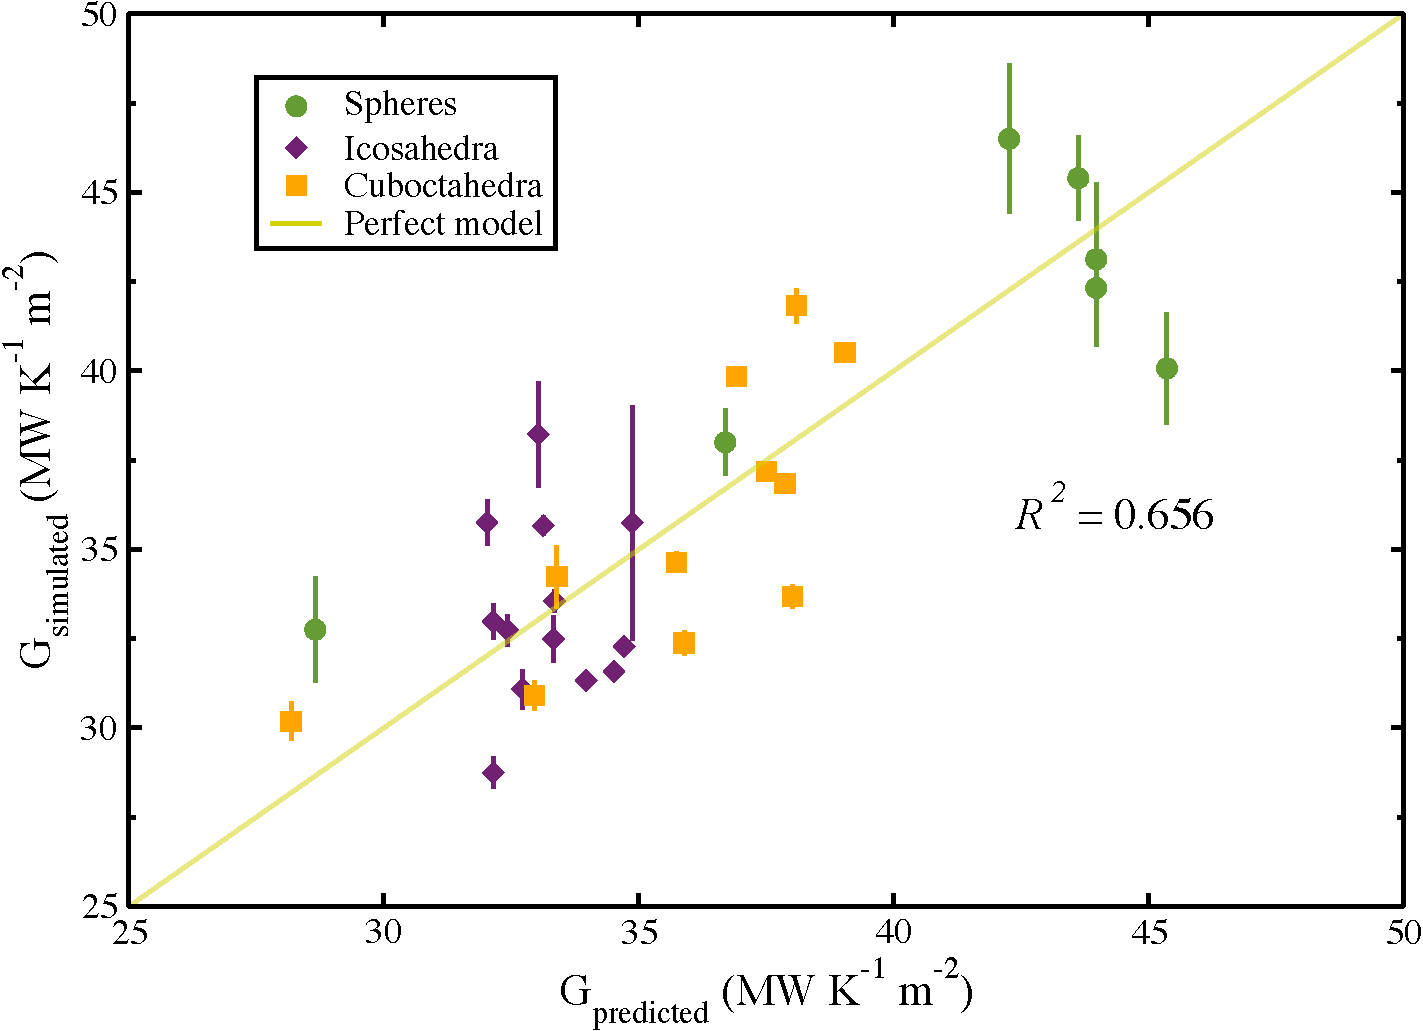
\includegraphics[width=\linewidth]{figures/models.pdf}
 	\caption{Structurally-predicted thermal conductance values from Eq. \eqref{eq:lin-fit} compared with the simulated thermal conductance values. Error bars indicate the standard error computed using five replica simulations. }
    \label{fig:models}
\end{figure}

% The vibrational density of states (VDOS) of the materials at the interface calculates the occupied low frequency phonon modes of the materials.
% As the radii of the particles increases, the VDOS of all gold atoms does not see a significant change below $100$ $cm^{-1}$ in either of the spherical systems, as seen in Supporting Information. 




\subsection{Conclusions}
The primary observation of this work is that particle morphology has a
significant effect on interfacial thermal conductance from bare
particles to the surrounding solvent.  In particular, spherical and
cuboctahedra particles have a size-dependent interfacial thermal
conductance, while icosahedral particles conduct heat to the
surrounding solvent only slightly better than the flat (111) facets.

This work explored one explanation for this difference in terms of the
density of undercoordinated sites on the surfaces of these three
particle morphologies. Nanospheres, because they are carved out of an
underlying FCC lattice, expose significantly undercoordinated atoms
($\text{CN} = 6-8$) to the solvent. For very small spheres,
microfacets of (111), (100), and (110) dominate the surface, but for
larger particles, the density of undercoordinated atoms becomes a
significant fraction of the exposed atoms.  In large icosahedral
particles, the particles are dominated by (111) faces, and the
$\text{CN} = 9$ atoms dominate the surface.  Similarly, in large
cuboctahedral particles, the (111) and (100) facets are both present,
and the $\text{CN} = 9$ and $\text{CN} = 8$ atoms share the particle
surface in a 2:3 ratio. Surface atom undercoordination leads directly
to changes in the surface vibrational density of states, particularly
at frequencies around $\sim 150 \text{~cm}^{-1}$.  The linear model
suggests that differences in surface atom undercoordination
(particularly for atoms that are undercoordinated relative to a flat
facet) may be largely responsible for our observations.

This is not a complete explanation for the conductance values,
however, as the large icosahedral particles exhibit $G$ values above
the planar (111) facet, and large cuboctahedra have $G$ values above
\textit{both} the (111) and (100) facets.  Edge and vertex atoms in
these clusters may play an outsized role, and collective low-frequency
modes of the particles may also be important, as the underlying
``bulk'' density of states also depends on particle morphology.

%Transmission models should therefore take both surface coordination and surface proximity into account when estimating energy transfer between materials.
%%%%%%%%%%%%%%%%%%%%%%%%%%%%%%%%%%%%%%%%%%%%%%%%%%%%%%%%%%%%%%%%%%%%%%%%%%%%%%%%%%%
%		COMPUTATIONAL DETAILS
%%%%%%%%%%%%%%%%%%%%%%%%%%%%%%%%%%%%%%%%%%%%%%%%%%%%%%%%%%%%%%%%%%%%%%%%%%%%%%%%%%%


%\begin{acknowledgement}
%  Support for this project was provided by the National Science
%  Foundation under grant CHE-1362211 and CHE-1663773. Computational
%  time was provided by the Center for Research Computing (CRC) at the
%  University of Notre Dame.
%\end{acknowledgement}
%
%\begin{suppinfo}
  %Details of system composition, surface densities of undercoordinated
  %atoms for ideal particle geometries, vibrational densities of states
  %for undercoordinated sites, fractional FCC ordering for particles,
 % and information on the linear model for thermal conductance.
%\end{suppinfo}

%\newpage

%\bibliography{Morph}

%\end{document}
